% ============================================================================
% ADVANCED FIXED INCOME -- Elaborato di gruppo ("Market microstructure insights")
% Identificazione dei regimi di liquidita' degli ETF tramite Hidden Markov Model
% Report metodologico completo: razionale, microstruttura ETF e NAV,
% misurazione della liquidita', l'HMM, stima, selezione del modello, e
% applicazione empirica a LQD.
% ============================================================================
\documentclass[11pt]{article}

\usepackage[margin=2.5cm]{geometry}
\emergencystretch=3em
\usepackage{amsmath,amssymb}
\usepackage{amsthm}
\usepackage{booktabs}
\usepackage{tikz}
\usepackage{pgfplots}
\pgfplotsset{compat=1.18}
\usetikzlibrary{arrows.meta,positioning,calc}
\usepackage{graphicx}
\usepackage{float}
\usepackage{xcolor}
\usepackage{listings}
\usepackage{hyperref}
\hypersetup{colorlinks=true, linkcolor=black, citecolor=black, urlcolor=blue!50!black}

\definecolor{pykeyword}{RGB}{0,0,180}
\definecolor{pystring}{RGB}{163,21,21}
\definecolor{pycomment}{RGB}{0,128,0}
\definecolor{pynumber}{RGB}{128,0,128}
\definecolor{pybackground}{RGB}{250,250,250}
\definecolor{pyframe}{RGB}{120,120,120}

\lstdefinestyle{pystyle}{
    language=Python,
    backgroundcolor=\color{pybackground},
    basicstyle=\ttfamily\footnotesize,
    keywordstyle=\color{pykeyword}\bfseries,
    commentstyle=\color{pycomment}\itshape,
    stringstyle=\color{pystring},
    numberstyle=\tiny\color{gray},
    identifierstyle=\color{black},
    showstringspaces=false,
    frame=single,
    framerule=0.4pt,
    rulecolor=\color{pyframe},
    breaklines=true,
    breakatwhitespace=false,
    columns=fullflexible,
    tabsize=4,
    numbers=left,
    numbersep=6pt,
    xleftmargin=1.2em,
    aboveskip=1em,
    belowskip=0.5em,
    morekeywords={as,with,lambda},
}
\lstset{style=pystyle}

\newtheorem{theorem}{Teorema}[section]
\newtheorem{proposition}[theorem]{Proposizione}
\newtheorem{corollary}[theorem]{Corollario}
\newtheorem{lemma}[theorem]{Lemma}
\newtheorem{algorithm}[theorem]{Algoritmo}
\theoremstyle{definition}
\newtheorem{definition}[theorem]{Definizione}
\theoremstyle{remark}
\newtheorem*{remark}{Osservazione}
\renewcommand{\proofname}{Dimostrazione}

\title{Identificazione dei Regimi di Liquidit\`a degli ETF tramite Hidden Markov Model}
\author{Tommaso Zeri \\ \small Advanced Fixed Income and Credit -- Elaborato di gruppo \\ \small Tema: \emph{Market microstructure insights}}
\date{Settembre 2026}

\begin{document}
\maketitle

\begin{abstract}
\noindent Gli exchange-traded fund (ETF) obbligazionari promettono una liquidit\`a continua, garantita dallo scambio, per una classe di attivi sottostante -- le obbligazioni corporate -- che invece si scambia per appuntamento, over the counter, a bassa frequenza. Questo disallineamento strutturale, talvolta chiamato \emph{liquidity transformation}, \`e di norma invisibile: nei mercati calmi l'arbitraggio di creazione/rimborso mantiene il prezzo di mercato dell'ETF ancorato al proprio Net Asset Value (NAV) entro pochi basis point. In condizioni di stress, l'arbitraggio pu\`o rompersi, il prezzo del fondo si scolla dal NAV, e gli intervalli di trading intraday si allargano bruscamente. Questo report sviluppa, da zero e con ogni passaggio matematico reso esplicito, un metodo interamente data-driven per rilevare questi episodi di stress di liquidit\`a: un Gaussian Hidden Markov Model (HMM) stimato su un piccolo insieme di feature giornaliere osservabili -- due proxy di volatilit\`a/illiquidit\`a basate su dati OHLCV e il premio/sconto assoluto (reale, non un proxy) del prezzo di mercato del fondo rispetto al proprio NAV -- che classifica ogni giorno di trading in un piccolo numero di regimi di liquidit\`a ordinati (Normal, Elevated, Shock), con il numero di regimi stesso scelto in modo oggettivo tramite il Bayesian Information Criterion (BIC). Deriviamo ogni componente della pipeline in dettaglio, a partire dalla teoria della probabilit\`a sottostante -- il teorema di Bayes, la stima di massima verosimiglianza, la propriet\`a di Markov, la densit\`a Gaussiana multivariata -- passando per il meccanismo di arbitraggio dell'ETF e la definizione del segnale di premio/sconto, i proxy di liquidit\`a e il razionale economico dietro ciascuno, il modello generativo dell'HMM, l'algoritmo di stima Baum--Welch (EM), il decoding di Viterbi, la selezione del modello tramite BIC, e un filtro di post-processing a isteresi. Applichiamo poi l'intera pipeline empiricamente a LQD (iShares iBoxx \$ Investment Grade Corporate Bond ETF), validandola su dati sintetici con un ground truth noto e, fuori campione, contro un calendario curato di episodi storici noti di stress di liquidit\`a; ed estendiamo l'analisi a un secondo segmento di credito, HYG (iShares iBoxx \$ High Yield Corporate Bond ETF), per verificare se i regimi di stress di liquidit\`a sono correlati, e si anticipano o ritardano a vicenda, tra lo spettro investment-grade/high-yield -- utilizzando uno score di stress continuo cross-HMM e un'analisi tramite cross-correlation function (CCF), essa stessa validata prima su una serie sintetica con un lead/lag noto e imposto, prima di essere applicata ai dati reali LQD/HYG.
\end{abstract}

\newpage
\tableofcontents
\newpage

% ============================================================================
\section{Introduzione}
\label{sec:intro}

\subsection{Motivazione e domanda di ricerca}

Un ETF obbligazionario corporate come LQD detiene un ampio paniere di singole obbligazioni corporate ed emette quote a fronte di quel paniere, scambiate in modo continuo su un mercato regolamentato come un'azione qualunque. Si tratta di una genuina innovazione per gli investitori: le singole obbligazioni corporate sono illiquide, si scambiano in lotti minimi ampi, e sono quotate (quando lo sono) tramite dealer run piuttosto che un order book centralizzato continuo. Un ETF racchiude centinaia di queste obbligazioni in un unico strumento a lotto piccolo, scambiato in borsa, liquido intraday.

La domanda economica che questo progetto pone \`e semplice da formulare e importante nella pratica: \emph{quella liquidit\`a intraday \`e genuina, oppure \`e presa in prestito dal mercato sottostante (illiquido) e rischia di sparire esattamente quando serve di pi\`u?} Lo shock COVID-19 di marzo 2020 ha dato una risposta drammatica e ben documentata -- LQD ha scambiato a sconto rispetto al proprio NAV di diversi punti percentuali per diversi giorni, anche se il meccanismo che dovrebbe prevenire esattamente questo (l'arbitraggio degli Authorized Participant) ha continuato a funzionare, solo a un ritmo pi\`u lento e costoso di quanto la quotazione continua in borsa dell'ETF suggerirebbe \cite{ohara2021anatomy}. L'obiettivo di questo progetto \`e trasformare quella narrazione qualitativa in una classificazione oggettiva, ripetibile, statisticamente fondata: per ogni giorno di trading nel campione, la liquidit\`a del fondo era \emph{Normal}, \emph{Elevated}, o in \emph{Shock} -- deciso non dal giudizio soggettivo di un analista o da una soglia arbitraria, ma da un modello probabilistico stimato sui dati stessi.

\subsection{Perch\'e un Hidden Markov Model}

Tre scelte di modellazione motivano l'approccio:
\begin{enumerate}
    \item \textbf{Regimi, non soglie.} Una soglia fissa (``volatilit\`a sopra $x\%$ \`e una crisi'') \`e arbitraria, specifica al campione, e cieca al fatto che lo stress di liquidit\`a \`e un \emph{fenomeno} multivariato e persistente, non una singola linea attraversata. Un HMM invece \emph{apprende} il numero e il carattere dei regimi dal comportamento congiunto di pi\`u feature rilevanti per la liquidit\`a simultaneamente.
    \item \textbf{La persistenza \`e un elemento di prima classe.} Le crisi di liquidit\`a non sono singoli giorni anomali isolati; sono episodi che durano da giorni a settimane, con una severit\`a autocorrelata. Una catena di Markov nascosta incorpora questa persistenza direttamente nel modello, tramite la sua matrice di transizione, invece di imporla come uno step di smoothing ad hoc a posteriori (un genuino modello a mistura i.i.d., al contrario, non ha memoria: non pu\`o distinguere un singolo giorno molto volatile circondato da giorni calmi da una crisi di pi\`u settimane).
    \item \textbf{Latente, non direttamente osservabile.} La ``liquidit\`a'' \`e un costrutto teorico -- non la osserviamo direttamente, solo le sue impronte nei dati di prezzo e volume (e, quando disponibile, nella deviazione del prezzo da un valore fondamentale come il NAV). Un modello a stati nascosti \`e esattamente l'oggetto formale corretto per una variabile che viene inferita da, ma non \`e uguale a, ci\`o che si osserva.
\end{enumerate}

\subsection{Contributo e struttura del report}

La Sezione~\ref{sec:prelim} raccoglie, da zero, ogni elemento di teoria della probabilit\`a usato nel resto del report -- probabilit\`a condizionata e teorema di Bayes, stima di massima verosimiglianza, la propriet\`a di Markov, e la distribuzione Gaussiana multivariata -- cos\`i che ogni derivazione successiva possa essere seguita senza consultare un riferimento esterno. La Sezione~\ref{sec:etf} espone la meccanica istituzionale della creazione/rimborso degli ETF e definisce formalmente il premio/sconto rispetto al NAV. La Sezione~\ref{sec:liquidity} ripercorre le dimensioni teoriche della liquidit\`a di mercato e deriva, in dettaglio, i tre proxy osservabili usati come input dell'HMM. La Sezione~\ref{sec:hmm} \`e il nucleo metodologico: la specificazione matematica completa dell'HMM Gaussiano, l'algoritmo di stima Baum--Welch, il decoding di Viterbi, la selezione del modello tramite BIC, e gli step di post-processing (riassegnazione delle etichette di stato, filtro a isteresi) necessari per trasformare una sequenza di stati decodificata grezza in una classificazione dei regimi economicamente interpretabile. La Sezione~\ref{sec:empirical} applica l'intera pipeline a LQD e documenta la strategia di validazione, incluso un controllo fuori campione contro un calendario di episodi noti di stress di mercato. La Sezione~\ref{sec:crossetf} estende l'analisi a un secondo segmento di credito, HYG, sviluppando uno score di stress continuo cross-HMM e una metodologia basata sulla cross-correlation function (CCF) per verificare relazioni di lead/lag tra i regimi di stress di liquidit\`a lungo lo spettro investment-grade/high-yield, validata prima su dati sintetici con un lag noto e imposto e poi applicata ai dati reali LQD/HYG. La Sezione~\ref{sec:limitations} discute limiti ed estensioni ulteriori. Un'appendice riproduce il codice core della pipeline e le run di validazione su dati sintetici usate per verificare l'implementazione prima di applicarla ai dati reali.

% ============================================================================
\section{Preliminari Matematici}
\label{sec:prelim}

Questa sezione raccoglie, in un unico posto e partendo da zero, ogni strumento probabilistico e statistico usato nel resto del report. Un lettore gi\`a a proprio agio con probabilit\`a condizionata, stima di massima verosimiglianza, catene di Markov e distribuzione Gaussiana multivariata pu\`o saltare direttamente alla Sezione~\ref{sec:etf}; a tutti gli altri consigliamo di leggere prima questa sezione, poich\'e ogni derivazione successiva del report vi si appoggia senza ripartire da zero.

\subsection{Variabili aleatorie, e probabilit\`a congiunta, marginale e condizionata}

Una \emph{variabile aleatoria} \`e una quantit\`a il cui valore non \`e noto con certezza in anticipo, ma \`e descritta da una distribuzione di probabilit\`a. Per una variabile aleatoria continua $X$, questa distribuzione \`e caratterizzata da una \emph{funzione di densit\`a di probabilit\`a} (pdf) $f_X(x)\ge0$ che soddisfa $\int_{-\infty}^{\infty}f_X(x)\,dx=1$, cos\`i che la probabilit\`a che $X$ cada in un intervallo \`e l'area sotto la densit\`a, $\mathbb{P}(a\le X\le b)=\int_a^b f_X(x)\,dx$. Per due variabili aleatorie $X,Y$ osservate insieme, la densit\`a \emph{congiunta} $f_{X,Y}(x,y)$ ne descrive il comportamento congiunto, e la densit\`a \emph{marginale} di $X$ da sola si recupera integrando (``sommando via'') $Y$: $f_X(x)=\int f_{X,Y}(x,y)\,dy$. Questo \`e l'analogo per variabili continue del fatto elementare, in probabilit\`a discreta, che $\mathbb{P}(A)=\sum_b\mathbb{P}(A,B=b)$ per qualunque partizione $\{B=b\}$ dello spazio campionario -- un fatto usato ripetutamente nella Sezione~\ref{sec:forward-backward} per ``marginalizzare via'' lo stato nascosto.

\begin{definition}[Probabilit\`a condizionata e teorema di Bayes]
Per due eventi $A,B$ con $\mathbb{P}(B)>0$, la probabilit\`a condizionata di $A$ \emph{dato} $B$ \`e definita come la probabilit\`a di $A$ ristretta al sotto-mondo in cui $B$ \`e noto essersi verificato, rinormalizzata cos\`i che $B$ stesso abbia probabilit\`a 1 in quel sotto-mondo:
\[
\mathbb{P}(A\mid B) := \frac{\mathbb{P}(A\cap B)}{\mathbb{P}(B)}.
\]
Riarrangiando questa definizione si ottiene $\mathbb{P}(A\cap B)=\mathbb{P}(A\mid B)\,\mathbb{P}(B)$; ma esattamente la stessa definizione applicata scambiando i ruoli di $A$ e $B$ d\`a $\mathbb{P}(A\cap B)=\mathbb{P}(B\mid A)\,\mathbb{P}(A)$. Poich\'e entrambe le espressioni sono uguali alla stessa quantit\`a $\mathbb{P}(A\cap B)$, sono uguali tra loro:
\[
\mathbb{P}(A\mid B)\,\mathbb{P}(B) = \mathbb{P}(B\mid A)\,\mathbb{P}(A) \qquad\Longrightarrow\qquad
\boxed{\ \mathbb{P}(A\mid B) = \frac{\mathbb{P}(B\mid A)\,\mathbb{P}(A)}{\mathbb{P}(B)}. \ }
\]
Questa ultima identit\`a \`e il \textbf{teorema di Bayes}. In parole: ci permette di convertire una probabilit\`a che possiamo specificare direttamente (qui, $\mathbb{P}(B\mid A)$) nella probabilit\`a condizionata ``invertita'' che vogliamo davvero ($\mathbb{P}(A\mid B)$), al costo di conoscere anche le due probabilit\`a marginali $\mathbb{P}(A)$ e $\mathbb{P}(B)$.
\end{definition}

Il teorema di Bayes \`e, letteralmente, l'identit\`a pi\`u usata in questo report. Ogni volta che la pipeline calcola la probabilit\`a di un regime di liquidit\`a nascosto \emph{dato} i dati osservati di prezzo/volume/NAV, \`e perch\'e il teorema di Bayes ci permette di invertire una probabilit\`a che l'HMM specifica direttamente per costruzione (la probabilit\`a di osservare certe feature \emph{dato} che il mercato \`e, poniamo, nel regime Shock) nella probabilit\`a che vogliamo davvero leggere su un grafico (la probabilit\`a che il mercato \emph{sia} nel regime Shock, dato ci\`o che abbiamo osservato). Le probabilit\`a smussate del Corollario~\ref{cor:smoothed} sono un'applicazione diretta, svolta per intero, esattamente di questa idea.

\subsection{Indipendenza e sequenze i.i.d.}

Due variabili aleatorie sono \emph{statisticamente indipendenti} se conoscere il valore dell'una non porta alcuna informazione sull'altra: formalmente, $\mathbb{P}(A\cap B)=\mathbb{P}(A)\,\mathbb{P}(B)$ per ogni coppia di eventi associati, il che per la definizione di probabilit\`a condizionata data sopra equivale a $\mathbb{P}(A\mid B)=\mathbb{P}(A)$ (condizionare su $B$ non sposta affatto la probabilit\`a di $A$). Una sequenza di variabili aleatorie $X_1,\dots,X_T$ \`e \textbf{indipendente e identicamente distribuita} (\emph{i.i.d.}) se ogni $X_t$ segue la stessa distribuzione e le variabili sono mutuamente indipendenti tra loro; l'indipendenza significa allora che la densit\`a congiunta si fattorizza in un semplice prodotto delle densit\`a (marginali) individuali,
\[
f(x_1,\dots,x_T) = \prod_{t=1}^{T}f(x_t).
\]
Questa fattorizzazione \`e esattamente ci\`o che rende trattabili computazionalmente le verosimiglianze di dati i.i.d.\ (Sezione~\ref{sec:mle} sotto). L'HMM Gaussiano della Sezione~\ref{sec:hmm} indebolisce deliberatamente questa assunzione: le feature osservate $x_1,\dots,x_T$ \emph{non} sono i.i.d.\ nel complesso (la loro distribuzione cambia nel tempo al cambiare del regime di liquidit\`a nascosto, e il regime stesso \`e correlato serialmente per costruzione), mentre una versione condizionata dell'assunzione i.i.d.\ viene mantenuta -- le osservazioni \emph{sono} indipendenti tra loro \emph{una volta noto l'intero percorso di stati nascosti} (la Sezione~\ref{sec:hmm-spec} rende questo preciso, ed \`e esattamente ci\`o che fa fattorizzare la verosimiglianza congiunta in quella sezione in un prodotto trattabile nonostante la dipendenza sottostante).

\subsection{Verosimiglianza e stima di massima verosimiglianza}
\label{sec:mle}

Data una famiglia parametrica di distribuzioni di probabilit\`a $f(x\mid\theta)$ indicizzata da un parametro incognito $\theta$ (che pu\`o essere uno scalare, un vettore, o -- come per l'HMM della Sezione~\ref{sec:hmm} -- un'intera collezione di vettori e matrici), e un campione osservato $x_1,\dots,x_T$, la \textbf{funzione di verosimiglianza} \`e definita come la densit\`a congiunta dei dati, ma vista come funzione dell'incognita $\theta$ per i dati effettivamente osservati (fissati), piuttosto che come funzione di $x$ per un $\theta$ fissato e noto:
\[
L(\theta) := f(x_1,\dots,x_T\mid\theta).
\]
L'intuizione \`e semplice: diversi valori candidati di $\theta$ rendono i dati che abbiamo effettivamente osservato pi\`u o meno probabili, e lo \textbf{stimatore di massima verosimiglianza} (MLE) \`e il valore del parametro che rende i dati osservati \emph{pi\`u} probabili,
\[
\widehat\theta_{MLE} = \arg\max_{\theta} L(\theta).
\]
Due semplificazioni pratiche standard ricorrono in tutto il report:
\begin{itemize}
    \item \textbf{Massimizzare la log-verosimiglianza invece della verosimiglianza.} Definiamo $\ell(\theta):=\ln L(\theta)$. Poich\'e il logaritmo naturale $\ln(\cdot)$ \`e una funzione strettamente crescente, preserva la posizione del massimo: $\arg\max_\theta L(\theta)=\arg\max_\theta \ell(\theta)$ (massimizzare una trasformazione crescente di una funzione non cambia mai quale input raggiunge il massimo). Il vantaggio pratico \`e numerico: per dati i.i.d.\ la verosimiglianza \`e un \emph{prodotto} di $T$ probabilit\`a, $L(\theta)=\prod_{t=1}^T f(x_t\mid\theta)$, ciascuna strettamente minore di uno, quindi $L(\theta)$ va in underflow a zero in virgola mobile gi\`a per $T$ moderatamente grandi (ad es.\ $0.1^{300}$ non \`e rappresentabile in doppia precisione); la log-verosimiglianza trasforma questo prodotto in una \emph{somma} numericamente stabile, $\ell(\theta)=\sum_{t=1}^T\ln f(x_t\mid\theta)$, che \`e esattamente la quantit\`a che ogni routine di stima in questo report (e ogni chiamata al metodo \texttt{.score()} di \texttt{hmmlearn} nel codice dell'appendice) calcola e restituisce realmente.
    \item \textbf{Massimizzazione iterativa, non in forma chiusa.} Per modelli i.i.d.\ semplici (ad es.\ stimare la media di un campione Gaussiano) $\widehat\theta_{MLE}$ ha una formula esplicita in forma chiusa ottenuta ponendo $\partial\ell/\partial\theta=0$ e risolvendo. Per modelli con struttura \emph{non osservata} (latente, nascosta) -- come l'HMM della Sezione~\ref{sec:hmm}, dove il percorso di regime nascosto $s_{1:T}$ non \`e mai osservato -- non esiste una forma chiusa, perch\'e la log-verosimiglianza coinvolge una somma \emph{dentro} il logaritmo (una somma su tutti i possibili percorsi nascosti) che non si semplifica algebricamente. $\widehat\theta_{MLE}$ si trova invece tramite un algoritmo numerico iterativo; l'algoritmo Expectation--Maximization (EM) della Sezione~\ref{sec:baumwelch} \`e esattamente una procedura di questo tipo, specializzata alla struttura particolare dell'HMM.
\end{itemize}

\subsection{Processi stocastici e la propriet\`a di Markov}
\label{sec:markov-prelim}

Un \textbf{processo stocastico} \`e semplicemente una sequenza di variabili aleatorie indicizzata dal tempo, $\{S_t\}_{t\ge1}$. Nella massima generalit\`a, senza alcuna assunzione semplificatrice, la distribuzione congiunta di $(S_1,\dots,S_T)$ pu\`o sempre essere decomposta tramite la \emph{regola a catena della probabilit\`a} (applicazione ripetuta della definizione di probabilit\`a condizionata data sopra),
\begin{align*}
\mathbb{P}(S_1,\dots,S_T) &= \mathbb{P}(S_1)\,\mathbb{P}(S_2\mid S_1)\,\mathbb{P}(S_3\mid S_1,S_2)\cdots\mathbb{P}(S_T\mid S_1,\dots,S_{T-1}) \\
&= \mathbb{P}(S_1)\prod_{t=2}^{T}\mathbb{P}(S_t\mid S_1,\dots,S_{t-1}),
\end{align*}
cio\`e la distribuzione di $S_t$ pu\`o, in generale, dipendere dall'\emph{intera} storia $S_1,\dots,S_{t-1}$ -- una decomposizione del tutto generale, ma praticamente inutile, poich\'e il numero di parametri necessari per specificare $\mathbb{P}(S_t\mid S_1,\dots,S_{t-1})$ per ogni possibile storia cresce esplosivamente con $t$.

\begin{definition}[Propriet\`a di Markov]
Un processo stocastico $\{S_t\}$ su uno spazio degli stati discreto ha la \textbf{propriet\`a di Markov} (\`e \emph{senza memoria}, o \emph{Markoviano del prim'ordine}) se, per ogni $t$, la distribuzione condizionata di $S_t$ data l'intera storia passata collassa a una dipendenza dal solo valore immediatamente precedente,
\[
\mathbb{P}(S_t\mid S_1,\dots,S_{t-1}) = \mathbb{P}(S_t\mid S_{t-1}).
\]
\end{definition}
Sostituendo questa relazione nella decomposizione generale a catena data sopra si ottiene una semplificazione drastica,
\[
\mathbb{P}(S_1,\dots,S_T) = \mathbb{P}(S_1)\prod_{t=2}^{T}\mathbb{P}(S_t\mid S_{t-1}),
\]
cos\`i che l'\emph{intera} distribuzione congiunta del processo \`e completamente determinata solo da (i) la distribuzione iniziale di $S_1$ e (ii) l'insieme delle probabilit\`a condizionate a un passo (di \emph{transizione}) $\mathbb{P}(S_t\mid S_{t-1})$ -- una semplificazione sfruttata in tutta la Sezione~\ref{sec:hmm}, e la giustificazione formale del perch\'e una catena di Markov necessiti solo di una distribuzione iniziale $\pi$ e di una matrice di transizione $A$ (Sezione~\ref{sec:hmm-spec}) per essere completamente specificata, invece di una tabella di probabilit\`a separata per ogni possibile storia. Una catena di Markov \`e \textbf{omogenea} (invariante nel tempo, o \emph{stazionaria} nelle sue dinamiche) se le probabilit\`a di transizione a un passo $\mathbb{P}(S_t=j\mid S_{t-1}=i)$ non dipendono esse stesse da $t$ -- l'assunzione mantenuta in tutto il report, che \`e ci\`o che permette a una \emph{singola}, fissa matrice $K\times K$ $A$ di descrivere le dinamiche della catena in ogni punto del campione, invece di una diversa matrice di transizione per ogni $t$.

\subsection{Notazione vettoriale e matriciale; matrici riga-stocastiche}

I simboli in minuscolo come $x_t\in\mathbb{R}^d$ denotano vettori colonna; $x^\top$ \`e la trasposta di $x$ (trasforma una colonna in una riga, usata per scrivere prodotti interni in forma compatta come $x^\top y=\sum_{k=1}^d x_ky_k$). Una matrice $A=(a_{ij})$ ha elemento $a_{ij}$ nella riga $i$, colonna $j$. Una matrice quadrata $A$ \`e \textbf{riga-stocastica} se ogni elemento \`e non negativo e ogni riga somma a uno, $a_{ij}\ge0$ e $\sum_{j}a_{ij}=1$ per ogni $i$ -- esattamente la condizione richiesta a una matrice di transizione Markoviana, poich\'e la riga $i$ di $A$ raccoglie l'intera distribuzione condizionata $\mathbb{P}(S_{t+1}=\cdot\mid S_t=i)$ sui $K$ possibili stati successivi, e ogni distribuzione di probabilit\`a valida deve avere essa stessa elementi non negativi che sommano a uno.

\subsection{La distribuzione Gaussiana multivariata}
\label{sec:mvgauss}

\begin{definition}[Densit\`a Gaussiana multivariata]
Un vettore aleatorio $d$-dimensionale $X$ segue una distribuzione Gaussiana (Normale) multivariata con vettore medio $\mu\in\mathbb{R}^d$ e matrice di covarianza $\Sigma\in\mathbb{R}^{d\times d}$ (simmetrica e definita positiva), scritto $X\sim\mathcal N(\mu,\Sigma)$, se la sua densit\`a \`e
\[
f(x\mid\mu,\Sigma) = \frac{1}{(2\pi)^{d/2}\,|\Sigma|^{1/2}}\exp\!\left(-\tfrac12(x-\mu)^\top\Sigma^{-1}(x-\mu)\right),
\]
dove $|\Sigma|$ denota il determinante di $\Sigma$ e $\Sigma^{-1}$ la sua inversa matriciale.
\end{definition}
Vale la pena rendere pienamente espliciti tre elementi di questa formula, poich\'e l'HMM della Sezione~\ref{sec:hmm} usa esattamente questa densit\`a -- una copia per ogni stato nascosto, ciascuna con i propri $\mu_i,\Sigma_i$ -- come distribuzione di emissione condizionata allo stato, e ogni verosimiglianza calcolata in questo report si riduce in ultima analisi a una valutazione di questa formula:
\begin{itemize}
    \item \textbf{La forma quadratica} $(x-\mu)^\top\Sigma^{-1}(x-\mu)$ \`e la \textbf{distanza di Mahalanobis} al quadrato del punto $x$ dalla media $\mu$. Generalizza l'ordinaria distanza euclidea al quadrato $\|x-\mu\|^2=(x-\mu)^\top(x-\mu)$ (che ne \`e il caso speciale $\Sigma=I$, la matrice identit\`a) per tenere conto del fatto che coordinate diverse di $X$ possono avere varianze diverse, e possono essere correlate tra loro -- entrambe catturate da $\Sigma$. Intuitivamente, un dato spostamento (euclideo) grezzo da $\mu$ \`e ``pi\`u sorprendente'' (densit\`a pi\`u bassa, distanza di Mahalanobis maggiore) in una direzione lungo cui $X$ \`e normalmente molto concentrata (bassa varianza) che in una direzione lungo cui $X$ \`e naturalmente dispersa (alta varianza); $\Sigma^{-1}$ \`e esattamente la trasformazione lineare che riscala gli spostamenti in base alla (inversa della) dispersione naturale della distribuzione in ogni direzione prima di misurare la distanza.
    \item \textbf{La costante di normalizzazione} $(2\pi)^{d/2}|\Sigma|^{1/2}$ al denominatore \`e precisamente il fattore che rende $\int_{\mathbb{R}^d}f(x\mid\mu,\Sigma)\,dx=1$, cio\`e che rende $f$ una densit\`a di probabilit\`a valida; non gioca alcun ruolo nel \emph{confrontare} la verosimiglianza relativa di un dato $x$ sotto due stati nascosti diversi $i,j$ dell'HMM, tranne nella misura in cui i due stati hanno matrici di covarianza diverse $\Sigma_i\ne\Sigma_j$ (e quindi costanti di normalizzazione diverse) -- uno stato la cui distribuzione di emissione \`e pi\`u dispersa (con $|\Sigma_i|$ maggiore) \`e, a parit\`a di altre condizioni, una distribuzione pi\`u diffusa, meno appuntita, che assegna densit\`a di picco pi\`u bassa anche alla propria media $\mu_i$.
    \item \textbf{Il caso speciale univariato.} Per $d=1$ (una singola feature, $\Sigma=\sigma^2$ una varianza scalare) la formula collassa nella familiare densit\`a Gaussiana univariata $f(x\mid\mu,\sigma^2)=\frac{1}{\sqrt{2\pi\sigma^2}}\exp\!\big(-\tfrac{(x-\mu)^2}{2\sigma^2}\big)$, che il lettore probabilmente gi\`a conosce; la versione multivariata \`e esattamente la generalizzazione naturale di questa formula a pi\`u feature distribuite congiuntamente, eventualmente correlate -- la situazione qui rilevante, poich\'e ogni regime di liquidit\`a nascosto \`e caratterizzato congiuntamente da $d\in\{2,3,4\}$ feature simultaneamente (Sezione~\ref{sec:feature-matrix}).
\end{itemize}

% ============================================================================
\section{Microstruttura di Mercato degli ETF e il Net Asset Value}
\label{sec:etf}

\subsection{Il meccanismo di creazione/rimborso}

Una quota di ETF non viene creata o distrutta dall'ordinario acquisto e vendita in borsa; gli ordinari scambi sul mercato secondario spostano semplicemente quote gi\`a esistenti tra investitori, esattamente come scambiare un'azione. Il \emph{numero di quote} del fondo cambia solo tramite un processo separato, di mercato primario, aperto a un piccolo insieme di grandi intermediari istituzionali chiamati \textbf{Authorized Participant} (AP). Due volte al giorno l'emittente pubblica un \emph{creation basket}: l'elenco esatto e la quantit\`a di obbligazioni sottostanti (o, per panieri meno liquidi, un mix di obbligazioni e cassa) che devono essere consegnate al fondo in cambio di un grande blocco di nuove quote ETF (una \emph{creation unit}, tipicamente 25.000--100.000 quote), e, simmetricamente, ci\`o che un AP che rimborsa riceve in cambio della consegna delle quote.

\begin{definition}[Creazione e rimborso]
Sia $NAV_t$ il Net Asset Value per quota del fondo al tempo $t$ (il valore di mercato del paniere obbligazionario sottostante diviso per le quote in circolazione) e $P_t$ il suo prezzo di mercato (scambiato in borsa) per quota.
\begin{itemize}
    \item \textbf{Creazione:} un AP assembla il paniere sottostante (che vale $NAV_t$ per quota, in aggregato), lo consegna all'emittente, e riceve in cambio nuove quote ETF. \`E profittevole ogni volta che $P_t>NAV_t$: l'AP pu\`o vendere immediatamente le nuove quote in borsa a un prezzo superiore al costo del paniere usato per crearle.
    \item \textbf{Rimborso:} un AP acquista quote ETF in borsa, le consegna all'emittente, e riceve in cambio il paniere sottostante (che vale $NAV_t$ per quota). \`E profittevole ogni volta che $P_t<NAV_t$: l'AP acquista quote a buon mercato e le rimborsa per un paniere che vale di pi\`u.
\end{itemize}
\end{definition}

Questo arbitraggio a doppio senso \`e precisamente ci\`o che dovrebbe mantenere $P_t$ ancorato vicino a $NAV_t$ in ogni momento: qualunque scarto persistente \`e, in linea di principio, un'opportunit\`a di profitto priva di rischio (o quasi, ignorando i costi di transazione e il piccolo rischio di timing di esecuzione dello scambio del paniere) per un AP, e la concorrenza tra AP dovrebbe far sparire lo scarto quasi immediatamente. La Figura~\ref{fig:creation-redemption} illustra le due gambe del meccanismo.

\begin{figure}[H]
\centering
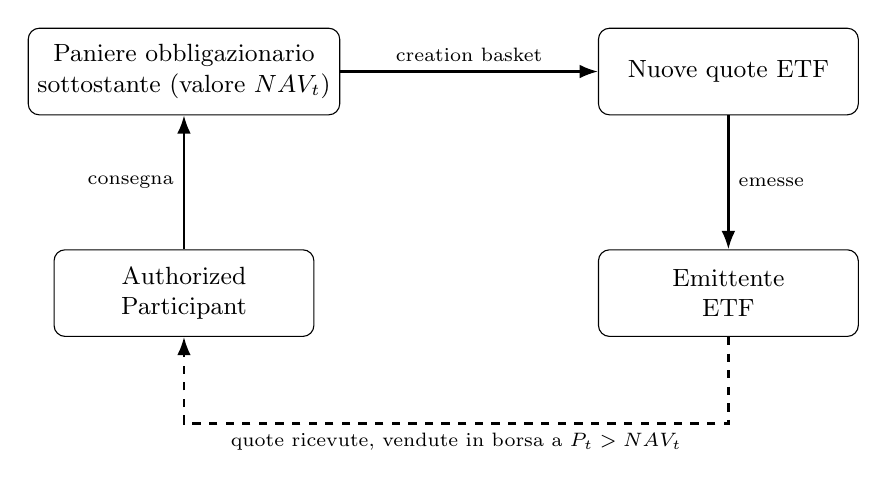
\begin{tikzpicture}[
    box/.style={draw, rounded corners, minimum width=3.3cm, minimum height=1.1cm, align=center, font=\small},
    arr/.style={-{Latex}, thick},
    node distance=3.6cm
]
\node[box] (ap) {Authorized\\Participant};
\node[box, right=of ap] (fund) {Emittente\\ETF};
\node[box, above=1.7cm of ap] (basket) {Paniere obbligazionario\\sottostante (valore $NAV_t$)};
\node[box, above=1.7cm of fund] (shares) {Nuove quote ETF};

\draw[arr] (ap.north) -- (basket.south) node[midway, left, font=\scriptsize] {consegna};
\draw[arr] (basket.east) -- (shares.west) node[midway, above, font=\scriptsize] {creation basket};
\draw[arr] (shares.south) -- (fund.north) node[midway, right, font=\scriptsize] {emesse};
\draw[arr, dashed] (fund.south) -- ($(fund.south)+(0,-1.1)$) -- ($(ap.south)+(0,-1.1)$) -- (ap.south);
\node[font=\scriptsize, align=center, below] at ($(ap.south)!0.5!(fund.south)+(0,-1.1)$)
    {quote ricevute, vendute in borsa a $P_t>NAV_t$};
\end{tikzpicture}
\caption{La gamba di creazione del meccanismo di arbitraggio: un AP consegna un paniere di obbligazioni sottostanti che vale $NAV_t$ per quota e riceve nuove quote ETF, vendute in borsa a $P_t$. Profittevole ogni volta che $P_t>NAV_t$. La gamba di rimborso inverte ogni freccia ed \`e profittevole ogni volta che $P_t<NAV_t$.}
\label{fig:creation-redemption}
\end{figure}

\subsection{Premio/sconto rispetto al NAV come segnale di stress di liquidit\`a}
\label{sec:premdisc}

\begin{definition}[Premio/sconto rispetto al NAV]
Il premio o sconto (con segno) del prezzo di mercato di un ETF rispetto al proprio NAV al tempo $t$ \`e
\[
\pi_t = \frac{P_t - NAV_t}{NAV_t} \times 100 \quad(\text{in \%}),
\]
con $\pi_t>0$ un premio (il fondo scambia sopra il valore delle proprie posizioni) e $\pi_t<0$ uno sconto (il fondo scambia a buon mercato). Ai fini di rilevare specificamente lo \emph{stress di liquidit\`a} -- in contrapposizione a una visione direzionale su quale lato del NAV il fondo si trovi -- l'oggetto rilevante \`e la magnitudine della dislocazione, non il suo segno:
\[
\boxed{\ \ell_t := |\pi_t| = \frac{|P_t - NAV_t|}{NAV_t}\times 100.\ }
\]
\end{definition}

\emph{Perch\'e questo \`e un segnale di liquidit\`a genuino (non un proxy).} In un mercato perfettamente liquido e senza frizioni, l'arbitraggio della Sezione~\ref{sec:etf} imporrebbe $\pi_t\equiv0$ in ogni momento. In pratica $\ell_t$ \`e piccolo ma strettamente positivo anche nei mercati calmi, e riflette (i) il bid-ask spread e i costi di transazione dell'assemblare/smontare un creation basket, (ii) il compenso dell'AP per il rischio di timing dell'esecuzione, e (iii) prezzi stantii o non sincroni delle obbligazioni sottostanti (illiquide) usate per calcolare $NAV_t$ stesso (i NAV obbligazionari sono tipicamente calcolati una volta al giorno da prezzi valutati/matrix price, mentre $P_t$ si aggiorna continuamente). Ci\`o che identifica un genuino episodio di stress di liquidit\`a \`e un \emph{allargamento brusco e sostenuto} di $\ell_t$ oltre questo livello di base: significa che (a) gli AP non sono pi\`u disposti o in grado di arbitraggiare lo scarto alla dimensione/costo usuali (vincoli di bilancio dei dealer, costi di transazione del paniere elevati, incertezza sul vero valore delle obbligazioni sottostanti illiquide), oppure (b) le obbligazioni sottostanti stesse hanno di fatto smesso di scambiare, cos\`i che $NAV_t$ \`e una stima stantia, che guarda al passato, in ritardo rispetto al repricing in tempo reale del rischio di credito che \`e invece riflesso quasi immediatamente nel $P_t$ scambiato continuamente. Entrambe le interpretazioni puntano allo stesso fenomeno sottostante: la liquidit\`a intraday pubblicizzata del fondo si \`e, almeno temporaneamente, scollata dalla liquidit\`a di ci\`o che effettivamente detiene -- che \`e esattamente l'oggetto che questo progetto si propone di rilevare. A differenza dei due proxy basati su OHLCV introdotti nella Sezione~\ref{sec:liquidity}, $\ell_t$ non \`e un proxy statistico indiretto per lo stress di liquidit\`a: \`e una misurazione diretta, model-free, della rottura del meccanismo di arbitraggio stesso.

\subsection{Fonte dei dati}

$P_t$ (come Close, insieme a Open/High/Low/Volume) proviene da dati OHLCV giornalieri di borsa (Yahoo Finance). $NAV_t$ proviene direttamente dalla storia giornaliera del NAV pubblicata dall'emittente del fondo stesso (fund page di iShares, export ``Historical''), che \`e la fonte autorevole usata dal meccanismo di arbitraggio stesso -- in contrapposizione a una stima del NAV ricostruita dai prezzi (valutati) delle obbligazioni sottostanti stesse, che reintrodurrebbe esattamente il tipo di rischio di proxy/stima che l'uso del segnale $\ell_t$ del fondo stesso \`e pensato per evitare.

% ============================================================================
\section{Misurare la Liquidit\`a}
\label{sec:liquidity}

\subsection{Dimensioni della liquidit\`a di mercato}

La teoria della microstruttura di mercato scompone la ``liquidit\`a'' -- un concetto intrinsecamente multidimensionale -- in diverse dimensioni complementari \cite{kyle1985continuous}:
\begin{itemize}
    \item \textbf{Tightness (ampiezza):} il costo di eseguire un piccolo scambio di andata e ritorno immediato -- tipicamente misurato dal bid-ask spread.
    \item \textbf{Depth (profondit\`a):} la dimensione che pu\`o essere scambiata al prezzo quotato corrente, o vicino ad esso, senza muoverlo.
    \item \textbf{Resiliency (resilienza):} la velocit\`a con cui il prezzo si riprende, e la profondit\`a si ricostituisce, dopo uno scambio che consuma liquidit\`a o uno shock.
    \item \textbf{Immediacy (immediatezza):} la velocit\`a con cui uno scambio di una data dimensione pu\`o essere eseguito del tutto.
\end{itemize}
Un mercato \`e ``illiquido'', nel senso rilevante per questo progetto, quando tightness e depth si deteriorano e la resiliency rallenta -- esattamente le condizioni sotto cui il meccanismo di arbitraggio dell'ETF della Sezione~\ref{sec:etf} diventa costoso o lento da eseguire, e sotto cui le obbligazioni sottostanti stesse diventano difficili da scambiare a un prezzo rappresentativo.

\subsection{Il problema del proxy}

Nessuna delle quattro dimensioni sopra \`e direttamente osservabile da dati OHLCV giornalieri: bid-ask spread e profondit\`a dell'order book richiedono dati di quotazione/scambio intraday (ad es.\ TAQ), che sono indisponibili oppure riservati dietro abbonamenti a dati istituzionali (la Sezione~\ref{sec:limitations} discute esplicitamente questo vincolo). La risposta standard nella letteratura empirica di microstruttura \`e costruire \emph{proxy}: statistiche calcolabili da dati giornalieri di prezzo/volume liberamente disponibili che sono teoricamente ed empiricamente correlate con le vere dimensioni (non osservate) di liquidit\`a sopra. Questo progetto usa due proxy di questo tipo basati su OHLCV, uno per tightness/volatilit\`a e uno per depth/price-impact, integrati dal segnale genuinamente diretto della Sezione~\ref{sec:premdisc}.

\subsection{Volatilit\`a basata sul range di Parkinson (1980)}
\label{sec:parkinson}

\begin{definition}[Stimatore di volatilit\`a di Parkinson]
Siano $H_t,L_t$ i prezzi high e low del giorno $t$. Lo stimatore di Parkinson della volatilit\`a realizzata del giorno \`e
\[
\sigma^{P}_t = \sqrt{\frac{1}{4\ln 2}\left(\ln\frac{H_t}{L_t}\right)^2}.
\]
\end{definition}

\paragraph{Impostazione.} Assumiamo che il log-prezzo intraday segua un moto Browniano senza drift (processo di Wiener) durante il giorno di trading, riscalato all'intervallo unitario $u\in[0,1]$:
\[
d\ln S_u = \sigma\,dW_u, \qquad \ln S_0 = 0,
\]
dove $W_u$ \`e un moto Browniano standard ($W_0=0$, incrementi Gaussiani indipendenti, $W_u-W_v\sim\mathcal N(0,u-v)$ per $u>v$) e $\sigma^2$ \`e il tasso di varianza istantanea (costante, da stimare) del log-prezzo. ``Senza drift'' significa che ignoriamo il drift atteso del log-prezzo su un singolo giorno, che \`e una quantit\`a minuscola rispetto alla sua varianza intraday e non influisce in modo rilevante sulla distribuzione del range.

\paragraph{Perch\'e il range del giorno \`e informativo su $\sigma$.} Un singolo rendimento close-to-close sul giorno, $\ln S_1-\ln S_0=\sigma W_1\sim\mathcal N(0,\sigma^2)$, \`e uno stimatore non distorto ma rumoroso (ad alta varianza) di $\sigma^2$: ``vede'' solo i due estremi del percorso. Il \textbf{range} del giorno, al contrario,
\[
R := \ln\!\Big(\max_{u\in[0,1]}S_u\Big/\min_{u\in[0,1]}S_u\Big) = \ln H-\ln L = \ln\frac{H}{L},
\]
usa l'intera escursione del percorso, non solo i suoi estremi, e quindi porta strettamente pi\`u informazione su $\sigma$ a parit\`a di un giorno di dati.

\paragraph{Derivazione.} \cite{parkinson1980} deriva la distribuzione esatta del range $R$ di un moto Browniano senza drift su $[0,1]$ usando il \emph{principio di riflessione} (un risultato classico: la distribuzione del massimo corrente di un moto Browniano iniziato in $0$ \`e uguale, per simmetria, a quella di $|W_u|$, poich\'e qualunque percorso che si riflette su una barriera al livello $m>0$ prima del tempo $u$ \`e esattamente altrettanto probabile della sua immagine speculare riflessa attorno a $m$) applicato congiuntamente al massimo e al minimo correnti. Dalla distribuzione del range risultante, Parkinson calcola il secondo momento in forma chiusa:
\[
\mathbb{E}\big[R^2\big] = 4\ln 2\,\sigma^2.
\]
Riarrangiando questa singola equazione per $\sigma^2$ si ottiene immediatamente lo stimatore naturale, non distorto, in stile metodo dei momenti, sostituendo il (non osservabile) secondo momento di popolazione $\mathbb{E}[R^2]$ con la singola realizzazione (osservata) $R^2$ stessa:
\[
\mathbb{E}[R^2]=4\ln2\,\sigma^2 \qquad\Longrightarrow\qquad \widehat{\sigma}^2 := \frac{R^2}{4\ln2} \quad\text{soddisfa}\quad \mathbb{E}[\widehat\sigma^2]=\sigma^2,
\]
cio\`e $\widehat\sigma^2$ \`e non distorto per il vero tasso di varianza $\sigma^2$ per costruzione, con la costante numerica $4\ln2\approx2.773$ che gioca esattamente il ruolo di un fattore di normalizzazione/riscalamento che converte il range quadrato atteso (pi\`u grande, essendo un massimo-meno-minimo invece di un singolo incremento) nella varianza correttamente scalata. Prendendo la radice quadrata di $\widehat\sigma^2$ e sostituendo $R=\ln H-\ln L=\ln(H/L)$ si ottiene lo stimatore di volatilit\`a di Parkinson enunciato nella definizione sopra,
\[
\sigma^P_t = \sqrt{\widehat\sigma^2} = \sqrt{\frac{1}{4\ln2}\Big(\ln\frac{H_t}{L_t}\Big)^2} = \frac{1}{2\sqrt{\ln2}}\left|\ln\frac{H_t}{L_t}\right|.
\]
Poich\'e sfrutta l'intero percorso del giorno invece dei soli due estremi, \cite{parkinson1980} mostra inoltre che lo stimatore \`e circa $5\times$ pi\`u efficiente statisticamente (cio\`e ha circa $1/5$ della varianza campionaria, a parit\`a di un giorno di dati) rispetto al rendimento close-to-close al quadrato sotto l'assunzione di diffusione mantenuta -- un guadagno di efficienza sostanziale che qui conta perch\'e $\sigma^P_t$ viene successivamente smussato e standardizzato (Sezione~\ref{sec:feature-matrix}) e usato come input giornaliero rumoroso dell'HMM, dove un ingrediente grezzo meno rumoroso si traduce direttamente in una feature meno rumorosa e pi\`u informativa.

\paragraph{Perch\'e fa da proxy per lo stress di liquidit\`a.} A parit\`a di rendimento close-to-close, un giorno con un ampio range High/Low rivela pi\`u frizione nella price discovery intraday -- scambi di andata e ritorno pi\`u ampi e rumorosi prima che il mercato si assesti -- rispetto a un giorno con un range stretto: esattamente la dimensione ``tightness'' della liquidit\`a sopra. Poich\'e usa l'intero range di trading del giorno invece dei soli due estremi, \`e anche uno stimatore di volatilit\`a sostanzialmente pi\`u efficiente statisticamente della volatilit\`a close-to-close per lo stesso scopo (il risultato di Parkinson stesso \`e circa un guadagno di efficienza $5\times$ sotto l'assunzione di diffusione mantenuta), il che conta quando lo stimatore stesso viene poi smussato e usato come input dell'HMM.

\subsection{Rapporto di illiquidit\`a di Amihud (2002)}
\label{sec:amihud}

\paragraph{Sfondo: il modello di price-impact di Kyle (1985).} Prima di definire il rapporto di Amihud, vale la pena esplicitare il semplice modello teorico di cui \`e pensato come proxy. \cite{kyle1985continuous} modella un market maker che osserva il flusso d'ordini totale $q$ (la quantit\`a netta acquistata, con segno positivo per acquisto netto e negativo per vendita netta) proveniente da un mix di trader informati e non informati (``rumore''), e fissa il prezzo come funzione lineare di quel flusso d'ordini,
\[
\Delta P = \lambda\, q,
\]
dove $\lambda>0$ (\textbf{lambda di Kyle}) \`e il \textbf{coefficiente di price-impact}: quanto si muove il prezzo per unit\`a di flusso d'ordini (netto, con segno). Il contenuto economico di $\lambda$ \`e esattamente la profondit\`a di mercato in negativo -- un $\lambda$ \emph{piccolo} significa che un grande flusso d'ordini $q$ pu\`o essere assorbito con solo un piccolo cambiamento di prezzo $\Delta P$ (un mercato profondo, liquido); un $\lambda$ \emph{grande} significa che anche un flusso d'ordini modesto muove il prezzo in modo sostanziale (un mercato sottile, illiquido, poich\'e il market maker deve essere compensato, tramite una risposta di prezzo pi\`u ripida, per il rischio aggiuntivo di scambiare con controparti potenzialmente meglio informate o di non riuscire a scaricare l'inventario risultante). $\lambda$ \`e quindi una misura diretta, basata su un modello, della dimensione ``depth'' della liquidit\`a introdotta nella Sezione~\ref{sec:liquidity} sopra.

\begin{definition}[Rapporto di illiquidit\`a di Amihud]
\[
ILLIQ_t = \frac{|r_t|}{DVOL_t}, \qquad r_t = \frac{P_t}{P_{t-1}}-1, \qquad DVOL_t = P_t\times Volume_t,
\]
cio\`e il rendimento giornaliero assoluto per dollaro di volume scambiato.
\end{definition}

\paragraph{Razionale.} $ILLIQ_t$ \`e il proxy empirico a bassa frequenza per eccellenza del coefficiente di price-impact di Kyle $\lambda$ sopra: dividere il cambiamento assoluto del prezzo del giorno $|r_t|$ (in percentuale) per il volume di scambio in dollari del giorno $DVOL_t$ produce esattamente l'analogo empirico su dati giornalieri di ``quanto si \`e mosso il prezzo, per dollaro di volume scambiato'' -- lo stesso oggetto concettuale di $\lambda=\Delta P/q$, solo misurato in unit\`a di rendimento percentuale su un intero giorno di flusso d'ordini aggregato invece che istantaneamente. Un mercato con liquidit\`a profonda e resiliente assorbe un dato volume in dollari di scambi con poco movimento di prezzo ($ILLIQ_t$ \emph{basso}, $\lambda$ basso); un mercato con liquidit\`a sottile si muove in modo sostanziale su un volume modesto ($ILLIQ_t$ \emph{alto}, $\lambda$ alto). \cite{amihud2002} mostra che questo semplice rapporto, pur richiedendo solo dati giornalieri di prezzo close-to-close e volume (nessun dato intraday di order book), correla fortemente nella pratica con misure di price-impact ben pi\`u intensive in dati, basate su microstruttura intraday, il che \`e precisamente il motivo per cui rimane il proxy di illiquidit\`a a bassa frequenza standard nella letteratura empirica di asset pricing e microstruttura, e il motivo per cui \`e una seconda feature di input naturale e liberamente calcolabile per l'HMM, accanto alla volatilit\`a di Parkinson della Sezione~\ref{sec:parkinson}.

\subsection{Z-score del volume}
\label{sec:volz}

\[
z^{vol}_t = \frac{Volume_t-\overline{Volume}_{t,w}}{s^{Volume}_{t,w}},
\]
il volume di scambio del giorno, standardizzato rispetto alla propria media e deviazione standard su una finestra mobile di $w$ giorni ($w=60$ giorni di trading in questo progetto). Le crisi di liquidit\`a sono frequentemente accompagnate da attivit\`a di scambio anomala (di solito elevata, occasionalmente collassata) rispetto alla norma recente del fondo stesso, quindi questa feature \`e inclusa come terzo segnale complementare basato sul volume. Come documentato nella Sezione~\ref{sec:empirical}, questa feature si \`e rivelata empiricamente \emph{non} discriminare bene tra i regimi per LQD ed \`e stata esclusa dal set di feature finale su questa base -- un esito che il workflow di confronto tra modelli basato su BIC della Sezione~\ref{sec:bic} \`e esplicitamente pensato per far emergere.

\subsection{Matrice delle feature e standardizzazione}
\label{sec:feature-matrix}

Le feature grezze $\{\sigma^P_t, ILLIQ_t, z^{vol}_t, \ell_t\}$ vivono su scale molto diverse, non stazionarie, e sono individualmente rumorose giorno per giorno. Due step di preprocessing vengono applicati prima che le feature vengano passate all'HMM:

\begin{enumerate}
    \item \textbf{Smoothing su finestra breve.} $\sigma^P_t$, $ILLIQ_t$ e $\ell_t$ vengono ciascuno sostituiti dalla propria media mobile semplice a 5 giorni, riducendo il rumore idiosincratico di un singolo giorno pur rispondendo entro circa una settimana di trading a un genuino cambio di regime.
    \item \textbf{Standardizzazione a finestra mobile.} Ogni feature smussata $x_t$ \`e standardizzata usando una finestra mobile di $w_z=252$ giorni di trading (un anno, con un minimo di 60 osservazioni prima che venga prodotto il primo valore standardizzato):
    \[
    \widetilde{x}_t = \frac{x_t - \mu_t^{w_z}}{s_t^{w_z}}, \qquad
    \mu_t^{w_z}=\frac{1}{w_z}\sum_{i=0}^{w_z-1}x_{t-i}, \qquad
    \big(s_t^{w_z}\big)^2=\frac{1}{w_z-1}\sum_{i=0}^{w_z-1}\big(x_{t-i}-\mu_t^{w_z}\big)^2.
    \]
    \emph{Cosa significa uno $z$-score, in termini semplici.} $\widetilde{x}_t$ esprime il valore grezzo della feature $x_t$ come ``quante deviazioni standard di distanza dalla propria media recente'' si trova attualmente l'osservazione -- $\widetilde{x}_t=0$ significa che $x_t$ \`e esattamente sulla propria media dell'ultimo anno, $\widetilde{x}_t=+2$ significa che $x_t$ \`e due deviazioni standard \emph{sopra} la propria norma recente (cio\`e insolitamente alto, rispetto alla storia recente del fondo stesso), e cos\`i via. Due propriet\`a di questa trasformazione contano per quanto segue: (i) \`e \emph{priva di unit\`a di misura} -- $\sigma^P_t$, $ILLIQ_t$ ed $\ell_t$ sono misurate in unit\`a interamente diverse, non confrontabili (una volatilit\`a, un rendimento-per-dollaro-di-volume, una deviazione percentuale dal NAV), e la densit\`a di emissione Gaussiana dell'HMM (Sezione~\ref{sec:mvgauss}) richiede che tutte le $d$ dimensioni di input siano su una scala numerica confrontabile perch\'e la matrice di covarianza $\Sigma_i$ sia ben condizionata e nessuna singola feature domini le altre semplicemente per via delle proprie unit\`a; e (ii) \`e \emph{auto-relativa} -- poich\'e $\mu_t^{w_z}$ e $s_t^{w_z}$ sono calcolati dalla finestra mobile del fondo stesso invece che da un benchmark esterno fisso, lo stesso valore standardizzato $\widetilde x_t=+2$ significa ``insolito per questo fondo, in questo momento, rispetto al proprio ultimo anno recente'' indipendentemente dal fatto che i livelli grezzi delle feature del fondo siano strutturalmente derivati (ad es.\ per un cambiamento della dimensione del fondo, per un cambiamento di regime di volatilit\`a a livello di mercato, o per un trend secolare pluriennale) -- la nozione appropriata di ``insolito'' per un esercizio di rilevamento di regimi che copre un decennio o pi\`u della storia di un singolo fondo.
\end{enumerate}
La standardizzazione \`e deliberatamente \emph{mobile}, non sull'intero campione: usare media e deviazione standard dell'intero campione per standardizzare un'osservazione all'inizio del campione farebbe trapelare informazione sul futuro (incluse crisi future) nel valore della feature per quell'osservazione -- una forma sottile di look-ahead bias che una finestra mobile evita per costruzione, al costo che le prime $w_z$ osservazioni del campione non siano disponibili per la stima del modello. La matrice delle feature standardizzata risultante $X=\{\widetilde{x}_t\}_{t=1}^{T}\in\mathbb{R}^{T\times d}$ ($d\in\{2,3,4\}$ a seconda di quali feature vengono mantenute) \`e l'input diretto dell'HMM della Sezione~\ref{sec:hmm}.

% ============================================================================
\section{Hidden Markov Model}
\label{sec:hmm}

\subsection{Specificazione formale}
\label{sec:hmm-spec}

\begin{definition}[Gaussian Hidden Markov Model]
Sia $\{S_t\}_{t=1}^{T}$ una catena di Markov a tempo discreto, del prim'ordine, omogenea, su uno spazio degli stati finito $\{1,\dots,K\}$ (i regimi di liquidit\`a \emph{nascosti}), completamente specificata da
\begin{itemize}
    \item una distribuzione iniziale $\pi=(\pi_1,\dots,\pi_K)$, $\pi_i=\mathbb{P}(S_1=i)$;
    \item una matrice di transizione riga-stocastica $K\times K$ $A=(a_{ij})$, $a_{ij}=\mathbb{P}(S_{t+1}=j\mid S_t=i)$, $\sum_j a_{ij}=1$.
\end{itemize}
Condizionatamente allo stato nascosto, il vettore di feature osservato (standardizzato) $X_t\in\mathbb{R}^d$ \`e estratto in modo indipendente tra i vari $t$ da una Gaussiana multivariata specifica dello stato:
\[
X_t \mid S_t=i \ \sim\ \mathcal{N}\big(\mu_i,\Sigma_i\big), \qquad
f(x\mid S_t=i) = \frac{1}{(2\pi)^{d/2}|\Sigma_i|^{1/2}}\exp\!\left(-\tfrac12(x-\mu_i)^\top\Sigma_i^{-1}(x-\mu_i)\right),
\]
con $\Sigma_i$ una matrice di covarianza $d\times d$ non vincolata (``full''), libera di differire tra gli stati. L'insieme dei parametri del modello \`e $\theta=(\pi,A,\{\mu_i,\Sigma_i\}_{i=1}^K)$.
\end{definition}

La verosimiglianza congiunta (dati completi) di un percorso nascosto $s_{1:T}=(s_1,\dots,s_T)$ e delle feature osservate $x_{1:T}$ \`e
\[
\mathbb{P}(s_{1:T},x_{1:T}\mid\theta) = \pi_{s_1}f(x_1\mid s_1)\prod_{t=2}^{T}a_{s_{t-1}s_t}\,f(x_t\mid s_t),
\]
e la verosimiglianza dei dati osservati (marginale) somma questa quantit\`a su ogni possibile percorso nascosto,
\[
\mathbb{P}(x_{1:T}\mid\theta) = \sum_{s_{1:T}\in\{1,\dots,K\}^T}\mathbb{P}(s_{1:T},x_{1:T}\mid\theta),
\]
una somma su $K^T$ percorsi che \`e computazionalmente infattibile da valutare direttamente per qualunque $T$ non banale; le ricorsioni forward-backward della Sezione~\ref{sec:forward-backward} la valutano invece in tempo $O(TK^2)$, tramite programmazione dinamica.

\subsection{Ricorsioni forward-backward}
\label{sec:forward-backward}

\begin{definition}[Variabili forward e backward]
\[
\alpha_t(i) := \mathbb{P}(x_1,\dots,x_t,S_t=i\mid\theta), \qquad
\beta_t(i) := \mathbb{P}(x_{t+1},\dots,x_T\mid S_t=i,\theta).
\]
\end{definition}

\begin{proposition}[Ricorsione forward]
\[
\alpha_1(i) = \pi_i\,f(x_1\mid i), \qquad
\alpha_{t+1}(j) = \left[\sum_{i=1}^K \alpha_t(i)\,a_{ij}\right]f(x_{t+1}\mid j), \qquad
\mathbb{P}(x_{1:T}\mid\theta) = \sum_{i=1}^K\alpha_T(i).
\]
\end{proposition}
\begin{proof}
\emph{Caso base.} Per definizione, $\alpha_1(i)=\mathbb{P}(x_1,S_1=i)=\mathbb{P}(S_1=i)\,\mathbb{P}(x_1\mid S_1=i)=\pi_i\,f(x_1\mid i)$, usando la definizione di probabilit\`a condizionata (Sezione~\ref{sec:prelim}) e direttamente la distribuzione iniziale e la densit\`a di emissione del modello.

\emph{Passo induttivo.} Assumiamo che $\alpha_t(i)=\mathbb{P}(x_{1:t},S_t=i)$ sia noto per ogni $i$; ne deriviamo $\alpha_{t+1}(j)$. Per prima cosa, introduciamo (marginalizziamo su) $S_t$ tramite la legge della probabilit\`a totale, scomponendo l'evento $\{x_{1:t+1},S_{t+1}=j\}$ a seconda di quale valore $S_t$ ha assunto:
\[
\alpha_{t+1}(j) = \mathbb{P}(x_{1:t+1},S_{t+1}=j) = \sum_{i=1}^K \mathbb{P}(x_{1:t},S_t=i,\,S_{t+1}=j,\,x_{t+1}).
\]
Ogni addendo \`e ora fattorizzato, tramite la regola a catena della probabilit\`a, in tre pezzi condizionati nell'ordine temporale naturale:
\begin{align*}
\mathbb{P}(x_{1:t},S_t=i,S_{t+1}=j,x_{t+1})
&= \underbrace{\mathbb{P}(x_{1:t},S_t=i)}_{=\ \alpha_t(i)}\\
&\quad\cdot\underbrace{\mathbb{P}(S_{t+1}=j\mid x_{1:t},S_t=i)}_{=\ \mathbb{P}(S_{t+1}=j\mid S_t=i)\ =\ a_{ij}\ \text{(propriet\`a di Markov)}}\\
&\quad\cdot\underbrace{\mathbb{P}(x_{t+1}\mid x_{1:t},S_t=i,S_{t+1}=j)}_{=\ f(x_{t+1}\mid j)\ \text{(indipendenza condizionata delle emissioni)}}.
\end{align*}
Il secondo fattore collassa ad $a_{ij}$ perch\'e la propriet\`a di Markov (Sezione~\ref{sec:markov-prelim}) dice che la transizione verso $S_{t+1}$ dipende solo da $S_t$, non dalla storia precedente $x_{1:t}$; il terzo fattore collassa a $f(x_{t+1}\mid j)$ perch\'e il modello generativo dell'HMM (Sezione~\ref{sec:hmm-spec}) specifica che $x_{t+1}$ dipende solo dallo stato nascosto \emph{corrente} $S_{t+1}=j$, ed \`e condizionatamente indipendente da tutto il resto (osservazioni passate, stati passati) dato quello stato. Sostituendo e raccogliendo $f(x_{t+1}\mid j)$ fuori dalla somma su $i$ (non dipende da $i$) si ottiene esattamente la ricorsione enunciata,
\[
\alpha_{t+1}(j) = \sum_{i=1}^K\alpha_t(i)\,a_{ij}\,f(x_{t+1}\mid j) = \left[\sum_{i=1}^K\alpha_t(i)\,a_{ij}\right]f(x_{t+1}\mid j).
\]
\emph{Terminazione.} Infine, $\sum_{i=1}^K\alpha_T(i)=\sum_i\mathbb{P}(x_{1:T},S_T=i)=\mathbb{P}(x_{1:T})$ per la legge della probabilit\`a totale, marginalizzando lo stato nascosto terminale $S_T$ (non pi\`u necessario, una volta che vogliamo solo la verosimiglianza dei dati osservati) -- questa \`e precisamente la verosimiglianza marginale della Sezione~\ref{sec:hmm-spec} che una somma bruta di $K^T$ termini richiederebbe altrimenti, qui ottenuta in $O(TK^2)$ operazioni (a ciascuno dei $T$ passi, calcolando $K$ nuovi valori di $\alpha$, ciascuno una somma su $K$ termini).
\end{proof}

\begin{proposition}[Ricorsione backward]
\[
\beta_T(i)=1\ \ \forall i, \qquad
\beta_t(i) = \sum_{j=1}^K a_{ij}\,f(x_{t+1}\mid j)\,\beta_{t+1}(j).
\]
\end{proposition}
\begin{proof}
\emph{Caso base.} $\beta_T(i)=\mathbb{P}(x_{T+1:T}\mid S_T=i)$ \`e, per convenzione, una probabilit\`a condizionata alle (vuote) ``osservazioni dopo $T$'' -- un prodotto vuoto, quindi identicamente $1$ per ogni $i$; \`e semplicemente una convenzione contabile che rende la ricorsione sotto autosufficiente per l'avvio.

\emph{Passo induttivo.} Assumiamo che $\beta_{t+1}(j)=\mathbb{P}(x_{t+2:T}\mid S_{t+1}=j)$ sia noto per ogni $j$. Introduciamo (condizioniamo su) $S_{t+1}$ tramite la legge della probabilit\`a totale, scomponendo sul suo possibile valore $j$:
\[
\beta_t(i) = \mathbb{P}(x_{t+1:T}\mid S_t=i) = \sum_{j=1}^K \mathbb{P}(S_{t+1}=j,\,x_{t+1},\,x_{t+2:T}\mid S_t=i).
\]
Ogni addendo si fattorizza, di nuovo tramite la regola a catena insieme alla propriet\`a di Markov e alla struttura di indipendenza condizionata delle emissioni:
\begin{align*}
\mathbb{P}(S_{t+1}=j,x_{t+1},x_{t+2:T}\mid S_t=i)
&= \underbrace{\mathbb{P}(S_{t+1}=j\mid S_t=i)}_{=\ a_{ij}}\cdot\underbrace{\mathbb{P}(x_{t+1}\mid S_{t+1}=j)}_{=\ f(x_{t+1}\mid j)}\cdot\underbrace{\mathbb{P}(x_{t+2:T}\mid S_{t+1}=j)}_{=\ \beta_{t+1}(j)},
\end{align*}
dove il terzo fattore usa il fatto che, una volta fissato $S_{t+1}=j$, le osservazioni future $x_{t+2:T}$ sono condizionatamente indipendenti da $S_t=i$ (tutta la ``memoria'' rilevante del passato \`e gi\`a riassunta da $S_{t+1}$, per la propriet\`a di Markov). Sommando su $j$ si ottiene esattamente la ricorsione enunciata. Come per il passo forward, questo calcola $\beta_t(i)$ per ogni $t,i$ in $O(TK^2)$ operazioni totali tramite programmazione dinamica, eseguita all'indietro nel tempo da $t=T$ fino a $t=1$.
\end{proof}

\begin{corollary}[Probabilit\`a di stato smussate]
\label{cor:smoothed}
\[
\gamma_t(i) := \mathbb{P}(S_t=i\mid x_{1:T},\theta) = \frac{\alpha_t(i)\,\beta_t(i)}{\sum_{k=1}^K\alpha_t(k)\,\beta_t(k)}.
\]
\end{corollary}
\begin{proof}
Per la definizione di probabilit\`a condizionata, $\gamma_t(i)=\mathbb{P}(S_t=i\mid x_{1:T})=\mathbb{P}(S_t=i,x_{1:T})/\mathbb{P}(x_{1:T})$. Scomponiamo la sequenza di osservazioni al numeratore al tempo $t$ nella sua parte passato-e-presente $x_{1:t}$ e nella sua parte futura $x_{t+1:T}$, e fattorizziamo usando la regola a catena e la struttura Markoviana esattamente come sopra:
\begin{align*}
\mathbb{P}(S_t=i,x_{1:T}) &= \mathbb{P}(x_{1:t},S_t=i)\cdot\mathbb{P}(x_{t+1:T}\mid x_{1:t},S_t=i) \\
&= \mathbb{P}(x_{1:t},S_t=i)\cdot\mathbb{P}(x_{t+1:T}\mid S_t=i) \\
&= \alpha_t(i)\,\beta_t(i),
\end{align*}
dove l'uguaglianza centrale elimina il condizionamento su $x_{1:t}$ nel secondo fattore perch\'e, per la propriet\`a di Markov, tutto ci\`o che \`e rilevante per le osservazioni future $x_{t+1:T}$ dato $S_t=i$ \`e gi\`a riassunto dallo stato corrente $S_t=i$ stesso -- le osservazioni passate $x_{1:t}$ non portano alcuna informazione aggiuntiva sul futuro una volta noto $S_t$. Dividendo per $\mathbb{P}(x_{1:T})=\sum_k\mathbb{P}(S_t=k,x_{1:T})=\sum_k\alpha_t(k)\beta_t(k)$ (di nuovo la legge della probabilit\`a totale, marginalizzando sui possibili valori di $S_t$) si ottiene la formula enunciata.
\end{proof}
\emph{Interpretazione.} $\gamma_t(i)$ risponde esattamente alla domanda per cui il teorema di Bayes (Sezione~\ref{sec:prelim}) \`e stato introdotto: dato \emph{tutto} ci\`o che \`e stato osservato (l'intero campione $x_{1:T}$), quanto \`e probabile che il mercato fosse nel regime di liquidit\`a $i$ nel giorno $t$? Queste sono le probabilit\`a di stato posteriori \emph{smussate} (sull'intero campione, a due passate -- una passata forward per $\alpha$, una passata backward per $\beta$) usate nella Sezione~\ref{sec:empirical} per tracciare la confidenza giorno per giorno del modello in ciascun regime, e nella Sezione~\ref{sec:crossetf} per costruire uno score di stress continuo cross-fondo. Sono concettualmente distinte dalla probabilit\`a \emph{filtrata} $\mathbb{P}(S_t=i\mid x_{1:t},\theta)\propto\alpha_t(i)$ (normalizzando solo $\alpha_t(i)$, senza la passata backward), che usa solo informazione disponibile fino a $t$ e sarebbe l'oggetto causale rilevante per un segnale di trading dal vivo, in tempo reale -- la Sezione~\ref{sec:limitations} torna su questa distinzione e sul perch\'e conta per trasformare questa pipeline in uno strumento di monitoraggio del rischio dal vivo.

\subsection{Stima dei parametri: l'algoritmo Baum--Welch (EM)}
\label{sec:baumwelch}

I parametri $\theta$ sono incogniti e devono essere stimati dai dati per massima verosimiglianza. Poich\'e il percorso nascosto non \`e osservato, la massimizzazione diretta di $\ell(\theta)=\ln\mathbb{P}(x_{1:T}\mid\theta)$ non ha forma chiusa (Sezione~\ref{sec:mle}): la verosimiglianza dei dati osservati coinvolge una somma su tutti i $K^T$ percorsi nascosti \emph{dentro} il logaritmo, che non si fattorizza in nulla che si possa differenziare e risolvere in forma chiusa. Questo si risolve con l'\textbf{algoritmo Expectation-Maximization (EM)}, specializzato agli HMM e noto in quel contesto come \textbf{algoritmo Baum--Welch} \cite{baum1970,rabiner1989}.

\paragraph{Il principio generale dell'EM.} Prima di specializzarci all'HMM, vale la pena capire \emph{perch\'e} l'EM funzioni in generale, per qualunque modello con dati non osservati. Sia $x$ i dati osservati e $s$ i dati non osservati (latenti) -- qui, $x=x_{1:T}$ e $s=s_{1:T}$, il percorso di stato nascosto -- e sia $q(s)$ \emph{qualunque} distribuzione di probabilit\`a sulla variabile latente. Partendo dalla log-verosimiglianza dei dati osservati e inserendo $q(s)/q(s)=1$ dentro la somma su $s$,
\[
\ell(\theta) = \ln\sum_s \mathbb{P}(x,s\mid\theta) = \ln\sum_s q(s)\,\frac{\mathbb{P}(x,s\mid\theta)}{q(s)}.
\]
Poich\'e $\ln(\cdot)$ \`e una funzione \emph{concava}, la disuguaglianza di Jensen afferma che il logaritmo di una media \`e almeno la media del logaritmo, $\ln\mathbb{E}[Y]\ge\mathbb{E}[\ln Y]$ per qualunque quantit\`a aleatoria $Y$; applicando questo con la media presa su $s\sim q(s)$ e $Y=\mathbb{P}(x,s\mid\theta)/q(s)$ si ottiene un limite inferiore sulla log-verosimiglianza, valido per \emph{qualunque} scelta di $q$:
\[
\ell(\theta) \ \ge\ \sum_s q(s)\,\ln\frac{\mathbb{P}(x,s\mid\theta)}{q(s)} \ =:\ \mathcal{L}(q,\theta) \qquad\text{(l'``evidence lower bound'', ELBO).}
\]
Un breve calcolo (usando il teorema di Bayes, Sezione~\ref{sec:prelim}, per scrivere $\mathbb{P}(x,s\mid\theta)=\mathbb{P}(s\mid x,\theta)\mathbb{P}(x\mid\theta)$) mostra che lo scarto tra $\ell(\theta)$ e il limite $\mathcal{L}(q,\theta)$ \`e esattamente una divergenza di Kullback--Leibler, $\ell(\theta)-\mathcal L(q,\theta)=\mathrm{KL}\big(q(s)\,\|\,\mathbb{P}(s\mid x,\theta)\big)\ge0$, che \`e zero precisamente quando $q(s)=\mathbb{P}(s\mid x,\theta)$ -- cio\`e il limite \`e \emph{stretto} esattamente quando $q$ \`e scelta come la vera posteriore della variabile latente sotto il $\theta$ corrente. Questo suggerisce immediatamente uno schema iterativo a due passi che dimostrabilmente non fa mai diminuire $\ell(\theta)$:
\begin{description}
    \item[Passo E] (Expectation): fissiamo $\theta=\theta^{(n)}$ al suo valore corrente e poniamo $q(s)=\mathbb{P}(s\mid x,\theta^{(n)})$ -- la posteriore sul percorso nascosto sotto i parametri correnti -- il che rende il limite stretto, $\mathcal L(q,\theta^{(n)})=\ell(\theta^{(n)})$, al $\theta^{(n)}$ corrente.
    \item[Passo M] (Maximization): con $q$ ora fissata (dal passo E), massimizziamo il limite $\mathcal L(q,\theta)$ rispetto a $\theta$ per ottenere $\theta^{(n+1)}=\arg\max_\theta\mathcal L(q,\theta)$.
\end{description}
Poich\'e $\ell(\theta^{(n+1)})\ge\mathcal L(q,\theta^{(n+1)})\ge\mathcal L(q,\theta^{(n)})=\ell(\theta^{(n)})$ (la prima disuguaglianza \`e il limite di Jensen applicato al nuovo $\theta^{(n+1)}$; la disuguaglianza centrale vale perch\'e il passo M \emph{massimizza} $\mathcal L$ rispetto a $\theta$, quindi il suo valore in $\theta^{(n+1)}$ non pu\`o essere pi\`u basso di quello nel vecchio $\theta^{(n)}$; l'uguaglianza finale \`e la strettezza del passo E), ogni iterazione EM \`e \emph{garantita} non far diminuire la log-verosimiglianza dei dati osservati -- la propriet\`a chiave che la rende una procedura di massima verosimiglianza valida (seppur solo localmente convergente). L'algoritmo Baum--Welch sotto \`e precisamente questa ricetta generale, specializzata all'HMM: la posteriore $q(s)=\mathbb{P}(s_{1:T}\mid x_{1:T},\theta^{(n)})$ del passo E \`e esattamente ci\`o che calcolano le ricorsioni forward-backward della Sezione~\ref{sec:forward-backward} (riassunte tramite le marginali $\gamma_t(i)$ e le marginali a coppie $\xi_t(i,j)$ sotto, che \`e tutto ci\`o di cui le formule del passo M hanno effettivamente bisogno), e la massimizzazione di $\mathcal L(q,\theta)$ rispetto a $\theta$ del passo M risulta avere, per la particolare struttura a famiglia esponenziale dell'HMM, la semplice soluzione in forma chiusa data sotto.

\begin{definition}[Probabilit\`a smussate a coppie]
\[
\xi_t(i,j) := \mathbb{P}(S_t=i,S_{t+1}=j\mid x_{1:T},\theta) = \frac{\alpha_t(i)\,a_{ij}\,f(x_{t+1}\mid j)\,\beta_{t+1}(j)}{\sum_{k=1}^K\sum_{l=1}^K\alpha_t(k)\,a_{kl}\,f(x_{t+1}\mid l)\,\beta_{t+1}(l)}.
\]
\end{definition}

\begin{algorithm}[Baum--Welch / EM]
\label{alg:baumwelch}
Partendo da una stima iniziale dei parametri $\theta^{(0)}$, si itera fino alla convergenza della log-verosimiglianza:
\begin{description}
    \item[Passo E.] Dato il $\theta^{(n)}$ corrente, si eseguono le ricorsioni forward-backward (Sezione~\ref{sec:forward-backward}) per calcolare $\gamma_t(i)$ e $\xi_t(i,j)$ per ogni $t,i,j$.
    \item[Passo M.] Si aggiornano i parametri in forma chiusa:
    \[
    \pi_i^{(n+1)} = \gamma_1(i), \qquad
    a_{ij}^{(n+1)} = \frac{\sum_{t=1}^{T-1}\xi_t(i,j)}{\sum_{t=1}^{T-1}\gamma_t(i)},
    \]
    \[
    \mu_i^{(n+1)} = \frac{\sum_{t=1}^{T}\gamma_t(i)\,x_t}{\sum_{t=1}^{T}\gamma_t(i)}, \qquad
    \Sigma_i^{(n+1)} = \frac{\sum_{t=1}^{T}\gamma_t(i)\,(x_t-\mu_i^{(n+1)})(x_t-\mu_i^{(n+1)})^\top}{\sum_{t=1}^{T}\gamma_t(i)}.
    \]
\end{description}
\end{algorithm}
\emph{Perch\'e queste particolari formule in forma chiusa.} Ricordando dalla verosimiglianza a dati completi (Sezione~\ref{sec:hmm-spec}) che $\ln\mathbb{P}(s_{1:T},x_{1:T}\mid\theta)=\ln\pi_{s_1}+\sum_{t=2}^T\ln a_{s_{t-1}s_t}+\sum_{t=1}^T\ln f(x_t\mid s_t)$ -- \emph{se} il percorso $s_{1:T}$ fosse effettivamente osservato, ciascuno dei tre pezzi (l'indicatore dello stato iniziale, i conteggi delle transizioni, le osservazioni per stato) potrebbe essere massimizzato \emph{separatamente} tramite MLE elementare: l'MLE di una multinomiale \`e la sua frequenza relativa osservata, e l'MLE di una Gaussiana sono la sua media e covarianza campionarie. Il passo M della ricetta EM generale della Sezione~\ref{sec:mle}, specializzato qui, massimizza il \emph{valore atteso} di questa stessa log-verosimiglianza a dati completi sotto la posteriore $q(s)=\mathbb{P}(s_{1:T}\mid x_{1:T},\theta^{(n)})$ calcolata nel passo E -- e poich\'e quel valore atteso \`e lineare in termini di indicatore del tipo ``la catena era nello stato $i$ al tempo $t$'', si riduce esattamente alle stesse formule MLE elementari che si userebbero con stati osservati, ma con ogni indicatore rigido 0/1 di appartenenza allo stato sostituito dalla propria controparte posteriore \emph{soffice}, frazionaria, $\gamma_t(i)$ (per gli aggiornamenti di distribuzione iniziale ed emissione) o $\xi_t(i,j)$ (per l'aggiornamento del conteggio delle transizioni). \`E esattamente ci\`o che mostrano le formule del passo M sopra: $a_{ij}^{(n+1)}$ \`e un rapporto tra conteggi (attesi) di transizioni $i\to j$ e visite (attese) totali a $i$, e $\mu_i^{(n+1)},\Sigma_i^{(n+1)}$ sono le ordinarie formule di media e covarianza campionarie, ma con ogni osservazione $x_t$ pesata dalla propria responsabilit\`a posteriore $\gamma_t(i)$ per lo stato $i$ invece che contata una volta per il proprio (non osservato) vero stato.

\emph{Convergenza.} Ogni iterazione EM \`e garantita, per l'argomento generale della Sezione~\ref{sec:mle} sopra, non far diminuire la log-verosimiglianza dei dati osservati $\ell(\theta)=\ln\mathbb{P}(x_{1:T}\mid\theta)$; in pratica l'algoritmo viene iterato finch\'e $\ell(\theta^{(n+1)})-\ell(\theta^{(n)})$ non scende sotto una piccola tolleranza ($10^{-4}$ nell'implementazione di questo progetto). L'algoritmo converge per\`o solo a un massimo \emph{locale} di $\ell(\theta)$: la superficie di verosimiglianza di un modello di tipo mistura come questo \`e generalmente multimodale in $\theta$ (permutare le $K$ etichette di stato, ad esempio, lascia $\ell(\theta)$ invariata, e possono esistere anche ottimi locali genuinamente diversi con interpretazioni economiche diverse), quindi la stima viene eseguita da $n_{init}=10$ inizializzazioni casuali indipendenti di $\theta^{(0)}$, e si mantiene la run che raggiunge la log-verosimiglianza convergente pi\`u alta -- una salvaguardia standard e semplice contro il rischio che una singola inizializzazione sfortunata finisca in un ottimo locale scadente.

\subsection{Decoding: l'algoritmo di Viterbi}
\label{sec:viterbi}

Una volta stimato $\widehat\theta$, la domanda naturale successiva \`e: qual \`e la singola sequenza di stati nascosti \emph{pi\`u probabile}, dato l'intero campione osservato? A questo risponde l'\textbf{algoritmo di Viterbi} \cite{viterbi1967}, un altro programma dinamico.

\begin{definition}[Variabile di Viterbi]
\[
\delta_t(i) := \max_{s_1,\dots,s_{t-1}}\mathbb{P}(s_1,\dots,s_{t-1},S_t=i,x_1,\dots,x_t\mid\theta),
\]
la probabilit\`a del singolo percorso migliore che termina nello stato $i$ al tempo $t$, congiuntamente alle osservazioni fino a $t$.
\end{definition}

\begin{proposition}[Ricorsione di Viterbi]
\[
\delta_1(i)=\pi_if(x_1\mid i), \qquad
\delta_{t+1}(j) = \Big[\max_{i}\ \delta_t(i)\,a_{ij}\Big]f(x_{t+1}\mid j), \qquad
\psi_{t+1}(j) = \arg\max_i\ \delta_t(i)\,a_{ij},
\]
con lo stato terminale ottimo e il percorso completo recuperati tramite backtracking:
\[
s_T^{\star}=\arg\max_i\delta_T(i), \qquad s_t^{\star}=\psi_{t+1}(s_{t+1}^{\star}),\ \ t=T-1,\dots,1.
\]
\end{proposition}
\emph{Schema.} Identica in struttura alla ricorsione forward, con la somma su $i$ (che marginalizza su tutti i possibili stati predecessori, poich\'e il passo forward vuole la probabilit\`a \emph{totale} di raggiungere $j$ per qualunque percorso) sostituita da un massimo su $i$ (che ottimizza sugli stati predecessori, poich\'e Viterbi vuole solo il \emph{singolo} percorso migliore). Questa sostituzione \`e un'istanza diretta del principio di ottimalit\`a di Bellman, l'argomento standard alla base di tutta la programmazione dinamica: il percorso migliore che termina in $(t+1,j)$ deve, ristretto ai suoi primi $t$ passi, essere esso stesso il percorso migliore verso \emph{qualche} $(t,i)$ -- perch\'e se esistesse un percorso strettamente migliore verso $(t,i)$, sostituirlo al posto del prefisso sub-ottimo produrrebbe un percorso strettamente migliore anche verso $(t+1,j)$, contraddicendo l'ottimalit\`a dell'originale. La ricorsione deve quindi solo provare ciascuno dei $K$ possibili stati predecessori $i$, moltiplicare per la corrispondente probabilit\`a di transizione $a_{ij}$, e mantenere il migliore (sia la probabilit\`a risultante $\delta_{t+1}(j)$ sia, tramite la variabile di tracciamento dell'argmax $\psi_{t+1}(j)$, \emph{quale} predecessore l'ha raggiunta, cos\`i che il percorso vincente possa essere ricostruito in seguito tramite backtracking).

\emph{Un'illustrazione minima svolta per intero.} Per rendere concreta la meccanica, consideriamo $K=2$ stati (Normal $=1$, Shock $=2$), $T=3$ giorni, matrice di transizione $A=\left(\begin{smallmatrix}0.9&0.1\\0.2&0.8\end{smallmatrix}\right)$, distribuzione iniziale $\pi=(0.9,0.1)$, e supponiamo che le densit\`a di emissione valutate sui tre vettori di feature osservati siano $f(x_1\mid 1)=0.5,\,f(x_1\mid2)=0.1$; $f(x_2\mid1)=0.2,\,f(x_2\mid2)=0.6$; $f(x_3\mid1)=0.3,\,f(x_3\mid2)=0.5$ (un giorno 2 che sembra insolitamente stressato, incastrato tra due giorni dall'aspetto pi\`u calmo). Allora: $\delta_1(1)=0.9\times0.5=0.45$, $\delta_1(2)=0.1\times0.1=0.01$; $\delta_2(1)=\max(0.45\times0.9,\,0.01\times0.2)\times0.2=0.405\times0.2=0.081$ (predecessore $i=1$), $\delta_2(2)=\max(0.45\times0.1,\,0.01\times0.8)\times0.6=0.045\times0.6=0.027$ (predecessore $i=1$); $\delta_3(1)=\max(0.081\times0.9,\,0.027\times0.2)\times0.3=0.0729\times0.3=0.02187$ (predecessore $i=1$), $\delta_3(2)=\max(0.081\times0.1,\,0.027\times0.8)\times0.5=0.0216\times0.5=0.0108$ (predecessore $i=2$). Poich\'e $\delta_3(1)>\delta_3(2)$, lo stato terminale ottimo \`e $s_3^\star=1$; il backtracking tramite $\psi$ d\`a $s_2^\star=\psi_3(1)=1$ e $s_1^\star=\psi_2(1)=1$ -- quindi il singolo percorso pi\`u probabile \`e $(1,1,1)$ (Normal per tutto il periodo), \emph{nonostante} la densit\`a di emissione del giorno 2 favorisca individualmente Shock ($f(x_2\mid2)=0.6>f(x_2\mid1)=0.2$): la forte persistenza del modello ($a_{11}=0.9$) e il fatto che l'evidenza del giorno 3 punti di nuovo verso Normal sono sufficienti, congiuntamente, a superare in peso il segnale isolato di un solo giorno. Questo \`e esattamente il comportamento qualitativo che il filtro a isteresi della Sezione~\ref{sec:hysteresis} rinforza esplicitamente, e precisamente il tipo di rumore di un singolo giorno che una regola a soglia ingenua (Sezione~\ref{sec:intro}) classificherebbe invece erroneamente.

Questo decoding \`e \textbf{sull'intero campione e retrospettivo}: sia $\delta_t(i)$ sia il percorso ricostruito tramite backtracking dipendono dall'intero campione osservato attraverso il $\widehat\theta$ stimato e, per ogni $t<T$, attraverso la ricorsione (che guarda avanti) che continua oltre $t$ (nell'esempio giocattolo, $s_1^\star$ e $s_2^\star$ sono stati determinati solo dopo aver incorporato anche l'evidenza del giorno 3). Risponde a ``guardando indietro sull'intero campione, quando il mercato era sotto stress di liquidit\`a'' -- non \`e un segnale filtrato, causale, utilizzabile per il trading dal vivo senza modifiche (Sezione~\ref{sec:limitations}).

\subsection{Selezione del modello: scegliere il numero di stati via BIC}
\label{sec:bic}

Il numero di stati nascosti $K$ \`e esso stesso incognito ed economicamente significativo (i dati supportano una semplice classificazione binaria Normal/Shock, oppure esiste un regime intermedio ``Elevated'' statisticamente distinguibile?). Poich\'e la log-verosimiglianza di un modello pi\`u ricco (a $K+1$ stati) non \`e mai inferiore a quella di un modello annidato a $K$ stati (un modello a $K$ stati \`e sempre recuperabile come caso speciale di un modello a $K+1$ stati, ad es.\ con le probabilit\`a di transizione di uno stato portate a zero, quindi la verosimiglianza \emph{massimizzata} del modello pi\`u ricco pu\`o solo essere almeno altrettanto grande), scegliere $K$ per sola massima verosimiglianza selezionerebbe sempre il $K$ pi\`u grande provato -- esattamente il problema di overfitting che la sola MLE non pu\`o risolvere, poich\'e premia qualunque aumento di flessibilit\`a anche quando quella flessibilit\`a sta adattandosi al rumore campionario invece che a struttura genuina.

\paragraph{Da dove viene la penalit\`a del BIC.} Un modo pienamente Bayesiano di confrontare due modelli candidati \`e confrontare le loro \textbf{verosimiglianze marginali} (dette anche \emph{model evidence}), $\mathbb{P}(x_{1:T}\mid K)=\int \mathbb{P}(x_{1:T}\mid\theta_K)\,p(\theta_K)\,d\theta_K$, che media la verosimiglianza su una prior $p(\theta_K)$ sui parametri del modello a $K$ stati invece di valutarla in un singolo punto stimato -- questo integrale penalizza automaticamente i modelli inutilmente flessibili, poich\'e spalmare la massa della prior su un $\theta_K$ di dimensione maggiore diluisce la verosimiglianza media a meno che la flessibilit\`a aggiuntiva non sia genuinamente supportata dai dati. \cite{schwarz1978} mostra che, per $T$ grande, questo integrale pu\`o essere approssimato tramite il \textbf{metodo di Laplace}: espandendo $\ln\big[\mathbb{P}(x_{1:T}\mid\theta_K)p(\theta_K)\big]$ in una serie di Taylor al second'ordine attorno al suo massimizzatore $\widehat\theta_K$ (approssimativamente l'MLE, per una prior ragionevolmente piatta) si trasforma l'integrando in una forma Gaussiana in $\theta_K$, il cui integrale \`e noto in forma chiusa; mantenendo solo i termini che crescono con $T$ (le costanti esatte dipendono dalla prior e svaniscono in importanza relativa per $T\to\infty$) si ottiene l'approssimazione asintotica
\[
\ln\mathbb{P}(x_{1:T}\mid K) \ \approx\ \ln\widehat{L}_K - \frac{p_K}{2}\ln T,
\]
dove $p_K=\dim(\theta_K)$ \`e il numero di parametri liberi (ogni parametro libero contribuisce una dimensione all'integrale di Laplace/Gaussiano, e ogni tale dimensione contribuisce un fattore dell'ordine $T^{-1/2}$ all'integrale approssimato, quindi $-\tfrac12\ln T$ per parametro su scala logaritmica). Moltiplicando per $-2$ (una normalizzazione che Schwarz scelse cos\`i che le differenze di BIC siano direttamente confrontabili con statistiche di due volte il rapporto di log-verosimiglianza, che sono asintoticamente distribuite come $\chi^2$ sotto condizioni di regolarit\`a standard) e invertendo la convenzione di segno cos\`i che il modello preferito \emph{minimizzi} invece di massimizzare il criterio si ottiene esattamente il \textbf{Bayesian Information Criterion}:
\[
BIC(K) := -2\ln\widehat{L}_K + p_K\ln T,
\]
dove $\widehat L_K=\mathbb{P}(x_{1:T}\mid\widehat\theta_K)$ \`e la verosimiglianza massimizzata (plug-in MLE) del modello a $K$ stati. I due termini bilanciano esattamente la tensione identificata sopra: $-2\ln\widehat L_K$ diminuisce (premiando l'adattamento) al crescere di $K$, mentre $p_K\ln T$ aumenta (penalizzando la complessit\`a) al crescere di $K$, e il modello selezionato \`e quello con il $BIC(K)$ pi\`u \emph{basso} -- il $K$ al quale aggiungere ulteriori stati smette di valere il proprio costo in parametri, data la dimensione del campione $T$ effettivamente disponibile. Si noti che la penalit\`a cresce con $\ln T$: con pi\`u dati, il criterio diventa progressivamente pi\`u disposto a tollerare parametri aggiuntivi, poich\'e un campione pi\`u lungo pu\`o stimarli con maggiore precisione -- una propriet\`a sensata per un criterio di selezione del modello.

\begin{proposition}[Conteggio dei parametri liberi, HMM Gaussiano a covarianza piena]
Per un HMM Gaussiano a $K$ stati con covarianza $d\times d$ non vincolata per stato,
\[
p_K = \underbrace{(K-1)}_{\text{dist.\ iniziale }\pi} + \underbrace{K(K-1)}_{\text{matrice di transizione }A} + \underbrace{Kd}_{\text{medie }\mu_i} + \underbrace{K\cdot\frac{d(d+1)}{2}}_{\text{covarianze }\Sigma_i}.
\]
\end{proposition}
\begin{proof}
\emph{Distribuzione iniziale $\pi$.} $\pi=(\pi_1,\dots,\pi_K)$ ha $K$ elementi, ma sono vincolati a essere non negativi e a sommare a uno, $\sum_i\pi_i=1$; questo singolo vincolo lineare elimina esattamente un grado di libert\`a (una volta scelti liberamente $\pi_1,\dots,\pi_{K-1}$, $\pi_K=1-\sum_{i<K}\pi_i$ \`e determinato), lasciando $K-1$ parametri liberi. Geometricamente, $\pi$ \`e vincolato a giacere sul \emph{simplesso di probabilit\`a} in $\mathbb{R}^K$, un oggetto $(K-1)$-dimensionale immerso in uno spazio $K$-dimensionale (esattamente analogo al fatto che tre probabilit\`a che sommano a uno tracciano un triangolo bidimensionale, non un volume tridimensionale).

\emph{Matrice di transizione $A$.} Ciascuna delle $K$ righe di $A$ \`e essa stessa una distribuzione di probabilit\`a (la riga $i$ \`e $\mathbb{P}(S_{t+1}=\cdot\mid S_t=i)$, Sezione~\ref{sec:markov-prelim}) e quindi, per l'argomento identico appena dato, giace sul proprio simplesso $(K-1)$-dimensionale, contribuendo $K-1$ parametri liberi; sommando sulle $K$ righe indipendenti si ottengono $K(K-1)$ parametri liberi per l'intera matrice.

\emph{Medie $\mu_i$.} Ciascuno dei $K$ vettori medi specifici per stato $\mu_i\in\mathbb{R}^d$ \`e non vincolato, contribuendo $d$ elementi liberi ciascuno, per $Kd$ totali.

\emph{Covarianze $\Sigma_i$.} Ciascuna $\Sigma_i$ \`e una matrice simmetrica $d\times d$ (solo la met\`a triangolare superiore, diagonale inclusa, \`e indipendente, poich\'e $\Sigma_{jk}=\Sigma_{kj}$) che deve inoltre essere definita positiva -- un vincolo di insieme aperto (esclude una frontiera di misura nulla di matrici degeneri) che non riduce il \emph{conteggio} dei parametri liberi, solo il loro intervallo ammesso. Il numero di elementi indipendenti nel triangolo superiore, diagonale inclusa, di una matrice $d\times d$ \`e $1+2+\cdots+d=\frac{d(d+1)}{2}$, quindi ciascuna $\Sigma_i$ contribuisce $\frac{d(d+1)}{2}$ parametri liberi, per $K\cdot\frac{d(d+1)}{2}$ totali.

Sommando i quattro blocchi (sono variazionalmente indipendenti tra loro, quindi i loro conteggi di parametri si sommano semplicemente) si ottiene il $p_K$ enunciato.
\end{proof}

\paragraph{Esempio svolto.} Per il set di feature effettivamente mantenuto nell'applicazione empirica sotto ($d=3$: volatilit\`a di Parkinson, illiquidit\`a di Amihud, e il segnale di premio/sconto -- Sezione~\ref{sec:empirical}), la formula d\`a, per i due valori candidati di $K$ confrontati in questo progetto:
\[
p_2 = \underbrace{1}_{K-1} + \underbrace{2}_{K(K-1)} + \underbrace{6}_{Kd} + \underbrace{12}_{K\cdot d(d+1)/2} = 21,
\qquad
p_3 = \underbrace{2}_{K-1} + \underbrace{6}_{K(K-1)} + \underbrace{9}_{Kd} + \underbrace{18}_{K\cdot d(d+1)/2} = 35,
\]
cio\`e il modello a 3 stati ha $35-21=14$ parametri liberi in pi\`u rispetto al modello a 2 stati -- un aumento sostanziale di flessibilit\`a (circa il $67\%$ di parametri in pi\`u) che la penalit\`a del BIC $p_K\ln T$ deve essere superata da un miglioramento corrispondentemente grande della log-verosimiglianza prima che il modello pi\`u ricco venga preferito; la Tabella~\ref{tab:results-template} riporta il confronto risultante $BIC(2)$ contro $BIC(3)$ sul campione reale di LQD.

I valori candidati $K\in\{2,3\}$ vengono confrontati in questo progetto (una suddivisione binaria Normal/Shock contro una suddivisione a tre vie Normal/Elevated/Shock), e il modello con BIC empiricamente pi\`u basso viene usato per il decoding finale -- la Sezione~\ref{sec:empirical} riporta il confronto.

\subsection{Riassegnazione delle etichette di stato}
\label{sec:relabel}

L'algoritmo EM della Sezione~\ref{sec:baumwelch} assegna gli \emph{indici} di stato $\{1,\dots,K\}$ in modo arbitrario: nulla nella procedura di stima garantisce che lo stato 1 sia il regime calmo. Gli stati vengono riassegnati, dopo la stima, ordinandoli secondo uno score di stress composito -- il vettore medio specifico per stato $\mu_i$ mediato sulle dimensioni delle feature (standardizzate, tutte crescenti con lo stress per costruzione),
\[
\text{stress}(i) = \frac1d\sum_{k=1}^d \mu_{i,k}, \qquad
\text{nuova etichetta di } i = \text{rango di stress}(i)\text{ tra }\{1,\dots,K\}\text{ (ascendente)},
\]
cos\`i che lo stato $0$ sia sempre il regime pi\`u calmo (Normal) e lo stato $K-1$ sia sempre il regime pi\`u stressato (Shock), con eventuali stati intermedi etichettati Elevated. Questa \`e puramente una convenzione contabile a posteriori (non cambia il modello stimato o il percorso decodificato, solo quale intero nomina quale stato) ma \`e essenziale per etichette di regime coerenti e confrontabili tra ticker diversi, campioni diversi, o ri-stime del modello.

\subsection{Filtro a isteresi (durata minima)}
\label{sec:hysteresis}

Il percorso di Viterbi grezzo della Sezione~\ref{sec:viterbi} pu\`o contenere escursioni isolate di uno o pochi giorni verso uno stato a stress pi\`u alto, guidate da un singolo giorno di trading insolitamente volatile piuttosto che da un genuino cambiamento sostenuto del regime di liquidit\`a sottostante. Poich\'e l'oggetto economico di interesse \`e un \emph{episodio} di liquidit\`a che dura da giorni a settimane, non un'etichetta tick-by-tick, un filtro deterministico di post-processing viene applicato sopra il percorso decodificato (gi\`a ottimo, nel senso di Viterbi).

\begin{algorithm}[Filtro a isteresi a durata minima]
\label{alg:hysteresis}
Dato un percorso di stati decodificato $s_{1:T}$ e una durata minima $m$: si identificano le sequenze massimali di stati identici consecutivi; finch\'e qualche sequenza ha lunghezza $<m$, si fonde la \emph{prima} tale sequenza breve con qualunque delle due sequenze vicine sia pi\`u lunga (una sequenza che tocca un confine del campione si fonde con l'unica vicina disponibile), e si ricalcola la decomposizione in sequenze; si ripete finch\'e ogni sequenza ha lunghezza $\ge m$ oppure l'intero percorso \`e una singola sequenza.
\end{algorithm}
Questo \`e uno step di smoothing applicato \emph{dopo} la stima e il decoding -- non ristima l'HMM n\'e altera $\widehat\theta$ -- ed \`e prassi standard ogniqualvolta un percorso di regime decodificato sia inteso come un piccolo numero di episodi discreti e persistenti. La Sezione~\ref{sec:empirical} usa $m=5$ giorni di trading.

% ============================================================================
\section{Applicazione Empirica a LQD}
\label{sec:empirical}

\subsection{Dati e campione}

Il target empirico \`e \textbf{LQD} (iShares iBoxx \$ Investment Grade Corporate Bond ETF), il pi\`u grande e liquido ETF obbligazionario corporate investment grade, scelto per due motivi: (i) \`e precisamente il tipo di fondo per cui la storia di liquidity transformation da creazione/rimborso della Sezione~\ref{sec:etf} \`e pi\`u rilevante (un ampio paniere diversificato di centinaia di obbligazioni individualmente illiquide), e (ii) entrambe le serie di dati richieste -- OHLCV giornaliero e storia ufficiale del NAV giornaliero -- sono liberamente disponibili per esso su un campione lungo (2015--oggi via Yahoo Finance e l'export ``Historical'' della fund page di iShares), senza richiedere un abbonamento a dati istituzionali riservato.

\subsection{Set di feature}

Seguendo le Sezioni~\ref{sec:parkinson}--\ref{sec:feature-matrix}, il set di feature candidato \`e $\{\sigma^P_t,\,ILLIQ_t,\,z^{vol}_t,\,\ell_t\}$ (smussato e standardizzato su finestra mobile). Come segnalato nella Sezione~\ref{sec:volz}, $z^{vol}_t$ si \`e rivelato empiricamente non separare bene i regimi stimati per LQD (le sue medie condizionate allo stato si sovrapponevano sostanzialmente tra i regimi, a differenza delle altre tre feature) ed \`e escluso dalla specificazione finale, lasciando il set a tre feature $\{\sigma^P_t,\,ILLIQ_t,\,\ell_t\}$ usato per i risultati sotto -- di per s\'e un punto metodologico utile: la selezione degli stati basata su BIC e l'ispezione delle distribuzioni delle feature condizionate allo stato (la Sezione~\ref{sec:appendix} mostra il grafico diagnostico corrispondente) forniscono insieme una base empirica, non puramente a priori, per la selezione delle feature.

\subsection{Confronto tra modelli e regimi stimati}

Gli HMM Gaussiani a $K\in\{2,3\}$ stati della Sezione~\ref{sec:hmm} vengono stimati sulla matrice standardizzata a 3 feature (ogni stima eseguita da $n_{init}=10$ inizializzazioni casuali, mantenendo la run a verosimiglianza pi\`u alta, come nella Sezione~\ref{sec:baumwelch}), il BIC della Sezione~\ref{sec:bic} viene calcolato per ciascuno, e il modello con BIC pi\`u basso viene selezionato per il decoding finale, la riassegnazione delle etichette (Sezione~\ref{sec:relabel}) e il filtro a isteresi con $m=5$ giorni (Sezione~\ref{sec:hysteresis}).

\begin{table}[H]
\centering
\caption{Struttura delle tabelle di confronto tra modelli e riepilogo dei regimi prodotte dalla pipeline (colonne come calcolate dal notebook allegato; popolare i valori numerici dalla run sui dati live del fondo).}
\label{tab:results-template}
\begin{tabular}{lccc}
\toprule
$K$ & Log-verosimiglianza & \# parametri $p_K$ & BIC \\
\midrule
2 & -- & $(2{-}1)+2(2{-}1)+2{\times}3+2{\times}\frac{3\cdot4}{2}=21$ & -- \\
3 & -- & $(3{-}1)+3(3{-}1)+3{\times}3+3{\times}\frac{3\cdot4}{2}=35$ & -- \\
\bottomrule
\end{tabular}
\end{table}

\begin{table}[H]
\centering
\caption{Struttura della tabella di riepilogo per regime (\% di giorni, persistenza media, e livelli medi standardizzati delle feature), come prodotta da \texttt{summarize\_regimes()} nel notebook allegato.}
\label{tab:regime-summary-template}
\begin{tabular}{lcccc}
\toprule
Regime & \% di giorni & Persistenza media (giorni) & media $\widetilde\sigma^P$ & media $\widetilde{ILLIQ}$ \\
\midrule
Normal & -- & -- & (pi\`u bassa) & (pi\`u bassa) \\
Elevated & -- & -- & (intermedia) & (intermedia) \\
Shock & -- & -- & (pi\`u alta) & (pi\`u alta) \\
\bottomrule
\end{tabular}
\end{table}

Per costruzione (Sezione~\ref{sec:relabel}), i livelli medi standardizzati delle feature sono monotonicamente crescenti da Normal a Shock per ogni feature mantenuta -- questo non viene testato ma imposto dalla convenzione di riassegnazione, ed \`e riportato qui per rendere esplicito esattamente ci\`o che quella convenzione garantisce rispetto a ci\`o che \`e un genuino risultato empirico (la \emph{persistenza}, la \emph{frequenza relativa}, e la \emph{struttura di transizione} dei regimi sono tutti output genuini del modello stimato, non artefatti della convenzione di etichettatura).

\subsection{Validazione fuori campione contro eventi di stress noti}
\label{sec:validation-events}

Un modello che recupera regimi statisticamente separati e persistenti \`e un controllo necessario ma non sufficiente: i regimi devono anche corrispondere a episodi \emph{economicamente reali}. Come controllo fuori campione -- il calendario sotto non \`e mai visto dall'HMM durante la stima -- il percorso di regime decodificato viene confrontato con un elenco curato di episodi noti di stress di liquidit\`a nel reddito fisso che coprono il periodo 2015--2025 (la dislocazione del mercato repo di settembre 2019, il crollo COVID-19 di marzo 2020 e l'annuncio della Federal Reserve delle proprie corporate credit facility, la crisi gilt/LDI del Regno Unito di settembre 2022, l'episodio di stress bancario regionale di marzo 2023 culminato nel salvataggio UBS--Credit Suisse, lo scioglimento dello yen carry-trade di agosto 2024, e il sell-off dei Treasury guidato dai dazi di aprile 2025, tra gli altri), chiedendosi se ciascun episodio noto cada dentro una finestra Elevated/Shock decodificata (entro una piccola tolleranza di $\pm5$ giorni di trading). Un tasso di successo elevato \`e evidenza che i regimi definiti statisticamente tracciano genuino stress di liquidit\`a documentato in modo indipendente, piuttosto che un artefatto della procedura di stima. La Figura~\ref{fig:events} (prodotta su dati sintetici per la validazione della pipeline; si veda la Sezione~\ref{sec:appendix}) mostra la meccanica di questo controllo.

\subsection{Grafici}

Le Figure~\ref{fig:main-chart}--\ref{fig:events} mostrano i grafici diagnostici e di classificazione dei regimi della pipeline. Per riproducibilit\`a all'interno di questo report sono generati sul dataset di validazione sintetico della Sezione~\ref{sec:appendix} (etichettato \texttt{DEMO}); il notebook Jupyter allegato produce i grafici identici sui dati reali LQD/NAV descritti sopra.

\begin{figure}[H]
\centering

\includegraphics[width=0.95\linewidth]{report_figs/demo_regimes_main.png}
\caption{Serie di prezzo con i regimi di liquidit\`a decodificati campiti sullo sfondo (severit\`a codificata come intensit\`a della campitura, una rampa ordinale a tinta unica, poich\'e i regimi sono ordinati per stress). Run di validazione sintetica.}
\label{fig:main-chart}
\end{figure}

\begin{figure}[H]
\centering

\includegraphics[width=0.95\linewidth]{report_figs/demo_regimes_detailed.png}
\caption{In alto: prezzo colorato per regime decodificato (Viterbi). In basso: probabilit\`a di stato posteriori smussate $\gamma_t(i)$ (Corollario~\ref{cor:smoothed}) come area impilata al 100\%, che mostra la confidenza giorno per giorno del modello in ciascun regime invece della sola etichetta decodificata rigida. Run di validazione sintetica.}
\label{fig:detailed-chart}
\end{figure}

\begin{figure}[H]
\centering

\includegraphics[width=0.62\linewidth]{report_figs/demo_transition_matrix.png}
\caption{Matrice di transizione stimata $\widehat A$ (Sezione~\ref{sec:baumwelch}), riordinata secondo l'etichettatura ascendente per stress della Sezione~\ref{sec:relabel}. Elementi diagonali elevati confermano che i regimi sono persistenti (una media di $1/(1-\widehat a_{ii})$ giorni per episodio), non rumore giorno per giorno. Run di validazione sintetica.}
\label{fig:transmat}
\end{figure}

\begin{figure}[H]
\centering

\includegraphics[width=0.95\linewidth]{report_figs/demo_regimes_vs_events.png}
\caption{Meccanica della validazione fuori campione della Sezione~\ref{sec:validation-events}: date di eventi di stress noti (marcatori numerati) sovrapposte al grafico di prezzo campito per regime decodificato. Run di validazione sintetica -- su dati sintetici il percorso di prezzo sottostante non ha relazione con eventi reali, quindi questa figura illustra solo il meccanismo di controllo, non un risultato genuino; il controllo su dati reali \`e riportato dal notebook allegato.}
\label{fig:events}
\end{figure}

% ============================================================================
\section{Confronto tra Segmenti di Credito: LQD contro HYG}
\label{sec:crossetf}

\subsection{Motivazione}

La pipeline delle Sezioni~\ref{sec:etf}--\ref{sec:hmm} \`e, per costruzione, interamente generica rispetto al ticker a cui viene applicata: nulla nella costruzione delle feature, nella specificazione dell'HMM, o nella macchina di stima/decoding \`e specifico a LQD. Questa sezione riutilizza la pipeline identica, non modificata, su un secondo fondo -- \textbf{HYG} (iShares iBoxx \$ High Yield Corporate Bond ETF), la controparte high-yield del focus investment-grade di LQD -- e pone una domanda economica genuinamente nuova che un'analisi su un singolo fondo non pu\`o rispondere: \emph{gli episodi di stress di liquidit\`a nel credito investment-grade e high-yield si muovono insieme, e se s\`i, lo stress di un segmento anticipa sistematicamente quello dell'altro?} Economicamente, gli emittenti high-yield sono pi\`u sensibili al rischio di credito e macroeconomico rispetto agli emittenti investment-grade, quindi un'ipotesi naturale \`e che la liquidit\`a high-yield debba deteriorarsi prima (o pi\`u severamente) quando lo stress sistemico si costruisce, con l'investment-grade che segue al diffondersi dell'avversione al rischio -- ma questa \`e una domanda empirica, non una conclusione scontata, e rispondervi rigorosamente richiede di confrontare due HMM stimati \emph{in modo indipendente}, il che solleva una genuina questione metodologica affrontata di seguito.

\subsection{Dalle etichette di regime discrete a uno score di stress continuo e confrontabile}
\label{sec:stress-score}

Gli HMM dei due fondi sono stimati in modo completamente indipendente l'uno dall'altro: ciascuno ha i propri parametri stimati $\widehat\theta^{LQD}$, $\widehat\theta^{HYG}$ (Sezione~\ref{sec:baumwelch}), il proprio numero di stati selezionato via BIC $K^{LQD}$, $K^{HYG}$ (Sezione~\ref{sec:bic}, non necessariamente uguali), e il proprio percorso di Viterbi decodificato (Sezione~\ref{sec:viterbi}). Correlare direttamente le etichette di regime \emph{discrete} dei due fondi non \`e quindi statisticamente significativo: l'indice di stato $2$ potrebbe essere ``Shock'' in una stima a 3 stati ma non esistere affatto in una stima a 2 stati, e anche quando entrambe le stime hanno per caso lo stesso $K$, l'etichetta discreta di Viterbi scarta la \emph{confidenza} giorno per giorno del modello, collassando una posteriore continua sottostante in un singolo intero rigido.

\begin{definition}[Score di stress continuo cross-fondo]
Per un fondo con un HMM stimato a $K$ stati e probabilit\`a di stato posteriori smussate $\gamma_t(k)$ (Corollario~\ref{cor:smoothed}), definiamo lo \textbf{score di stress} del giorno $t$ come l'indice di stato \emph{atteso} a posteriori,
\[
\mathrm{score}_t := \mathbb{E}[S_t\mid x_{1:T},\widehat\theta] = \sum_{k=0}^{K-1} k\cdot\gamma_t(k),
\]
usando l'etichettatura ascendente per stress della Sezione~\ref{sec:relabel} (stato $0=$ Normal, stato $K-1=$ Shock) cos\`i che $\mathrm{score}_t$ sia un numero reale in $[0,K-1]$ che si muove con continuit\`a (invece di saltare in modo discreto) tra il regime pi\`u calmo e quello pi\`u stressato, e rifletta l'intera incertezza posteriore del modello invece del solo stato singolo pi\`u probabile.
\end{definition}
Questa \`e semplicemente la definizione del valore atteso di una variabile aleatoria discreta ($S_t$, sotto la propria distribuzione posteriore $\gamma_t(\cdot)$) applicata direttamente -- un passo elementare ma importante, poich\'e \`e esattamente ci\`o che rende lo score confrontabile, nel proprio \emph{comovimento} (correlazione, lead/lag), tra due fondi i cui $K$ e $\widehat\theta$ sottostanti differiscono completamente: entrambi gli score sono costruiti dalla formula identica, applicata al proprio modello stimato di ciascun fondo. Vale la pena esplicitare una precisazione per rigore: se $K^{LQD}\ne K^{HYG}$, gli \emph{intervalli assoluti} dei due score $[0,K^{LQD}-1]$ e $[0,K^{HYG}-1]$ differiscono, quindi solo le statistiche di comovimento \emph{relativo} (correlazione, cross-correlazione, e un indicatore binario a soglia, tutti introdotti sotto) vengono confrontate in modo significativo tra fondi -- non, ad esempio, una differenza numerica diretta $\mathrm{score}_t^{LQD}-\mathrm{score}_t^{HYG}$, che confonderebbe una genuina differenza di livello di stress con una differenza dovuta semplicemente al numero di stati dei due modelli.

\subsection{Cross-correlation function (CCF) e stima del lead/lag}
\label{sec:ccf}

\begin{definition}[Cross-correlation function campionaria]
Per due serie temporali $a_t,b_t$ osservate su un insieme comune di date e un lag intero $\ell$, la \textbf{cross-correlation function} (Pearson) \cite{boxjenkins} al lag $\ell$ \`e il coefficiente di correlazione campionario ordinario tra $a_t$ e $b_t$ shiftata di $\ell$ periodi,
\[
CCF(\ell) := \mathrm{corr}\big(a_t,\,b_{t-\ell}\big) = \frac{\sum_t\big(a_t-\bar a\big)\big(b_{t-\ell}-\bar b\big)}{\sqrt{\sum_t(a_t-\bar a)^2}\sqrt{\sum_t(b_{t-\ell}-\bar b)^2}},
\]
valutata sul campione comune (sovrapposto, dopo lo shift) di date, per $\ell$ che varia su una finestra simmetrica $\ell\in\{-L,\dots,L\}$ (questo report usa $L=10$ giorni di trading). Il lead/lag stimato \`e $\widehat\ell^\star=\arg\max_\ell CCF(\ell)$, il lag al quale le due serie sono pi\`u simili.
\end{definition}

\paragraph{Convenzione di segno, derivata (non solo asserita).} \`E facile invertire per errore la direzione di interpretazione di $CCF(\ell)$, quindi vale la pena derivarla esplicitamente invece di limitarsi a enunciarla. Supponiamo, a scopo illustrativo, che lo score di stress di $b$ sia \emph{letteralmente} un'anteprima dello score di stress di $a$ tra $m$ giorni nel futuro, $b_t = a_{t+m}$ per ogni $t$ (una versione giocattolo, deterministica e senza rumore, di ``$b$ anticipa $a$ di $m$ giorni''). Riarrangiando, $a_t = b_{t-m}$: il valore \emph{odierno} di $a$ \`e uguale al valore di $b$ di $m$ giorni \emph{fa}. Sostituendo nella definizione di $CCF(\ell)$ sopra, la correlazione tra $a_t$ e $b_{t-\ell}$ \`e quindi \emph{esattamente} $1$ (una corrispondenza perfetta) precisamente quando $\ell=m$, poich\'e solo allora $b_{t-\ell}=b_{t-m}=a_t$ combacia perfettamente con se stesso; per qualunque altro $\ell$, $b_{t-\ell}$ confronta $a_t$ con un valore di $b$ del giorno sbagliato, e la correlazione \`e (genericamente) pi\`u bassa. Quindi: $CCF(\ell)$ che \textbf{raggiunge il picco a un valore positivo} $\widehat\ell^\star=m>0$ significa che $b_{t-m}$ combacia meglio con $a_t$, cio\`e \emph{il valore passato di $b$ ($m$ giorni fa) \`e ci\`o che si allinea con il valore presente di $a$} -- in altre parole, qualunque cosa $b$ abbia fatto $m$ giorni fa, $a$ la sta facendo ora: \textbf{$b$ anticipa $a$ di $m$ giorni}. Simmetricamente, un picco a un valore negativo $\widehat\ell^\star=-m<0$ significa che $a$ anticipa $b$ di $m$ giorni, e un picco a $\widehat\ell^\star=0$ significa che le due serie si muovono insieme in modo contemporaneo, senza lead/lag rilevabile alla frequenza giornaliera di questa analisi. Questo report pone sempre $a=$ lo score di stress di LQD e $b=$ lo score di stress di HYG, quindi un lag stimato positivo si legge, ovunque, come ``HYG anticipa LQD''.

\subsection{Comovimento oltre la correlazione: una diagnostica di lift su tabella di contingenza}
\label{sec:lift}

Correlazione e CCF riassumono il comovimento \emph{lineare, continuo} tra i due score; un controllo complementare, non parametrico, pone una domanda binaria pi\`u semplice: nei giorni in cui un fondo \`e ``stressato'', l'altro fondo \`e anch'esso insolitamente propenso a essere stressato, oltre a quanto il puro caso predirebbe?

\begin{definition}[Indicatore di stress e lift]
Fissiamo una soglia $c$ (questo report usa $c=0.5$, il punto medio tra Normal e il primo stato non-Normal) e definiamo gli indicatori binari di stress $D_t^{a}:=\mathbb{1}\{a_t>c\}$, $D_t^{b}:=\mathbb{1}\{b_t>c\}$. Siano $\widehat p_a=\overline{D^a}$, $\widehat p_b=\overline{D^b}$, $\widehat p_{ab}=\overline{D^aD^b}$ le frequenze empiriche (medie campionarie) marginali e congiunte di stress. Il \textbf{lift} \`e
\[
\mathrm{lift} := \frac{\widehat p_{ab}}{\widehat p_a\cdot\widehat p_b}.
\]
\end{definition}
\begin{proposition}
Sotto indipendenza statistica di $D^a_t$ e $D^b_t$, $\mathrm{lift}=1$ (in popolazione, cio\`e sostituendo le frequenze campionarie con le rispettive probabilit\`a di popolazione).
\end{proposition}
\begin{proof}
L'indipendenza dei due indicatori binari significa, per definizione (Sezione~\ref{sec:prelim}), $\mathbb{P}(D^a=1,D^b=1)=\mathbb{P}(D^a=1)\,\mathbb{P}(D^b=1)$. Sostituendo $p_{ab}=p_a\cdot p_b$ nella formula del lift si ottiene $\mathrm{lift}=p_a p_b/(p_a p_b)=1$.
\end{proof}
$\mathrm{lift}>1$ indica quindi che i due fondi sono stressati \emph{insieme} pi\`u spesso di quanto l'indipendenza predirebbe (comovimento in eccesso positivo); $\mathrm{lift}<1$ indicherebbe che i fondi sono stressati insieme \emph{meno} spesso del caso (un'associazione negativa, non attesa qui su basi economiche); $\mathrm{lift}\approx1$ indicherebbe nessun comovimento in eccesso rilevabile oltre a quanto le frequenze di stress marginali individuali dei due fondi da sole implicherebbero. A differenza di $CCF(0)$, il lift \`e calcolato sull'indicatore binario a soglia invece che sullo score continuo, ed \`e quindi una diagnostica genuinamente diversa (seppur correlata) -- riportata qui come controllo di robustezza sul risultato basato sulla correlazione, non come sua sostituzione.

\subsection{Validazione su dati sintetici con un lag noto e imposto}
\label{sec:crossetf-demo}

Seguendo la stessa filosofia di validazione del controllo sintetico su singolo fondo dell'appendice (Sezione~\ref{sec:appendix}), la metodologia di stima del lead/lag della Sezione~\ref{sec:ccf} viene prima validata su una serie sintetica accoppiata con un lag di ground truth \emph{noto}, prima di essere considerata affidabile sui dati reali LQD/HYG. Concretamente, viene generato un secondo ``fondo'' sintetico il cui percorso di regime vero (nascosto, ground truth) \`e costruito come il percorso di regime vero del \emph{primo} fondo sintetico, shiftato di $m=3$ giorni di trading nel futuro rispetto al calendario proprio del secondo fondo -- cio\`e, per costruzione, il regime vero del secondo fondo al tempo $t$ \`e uguale al regime vero del primo fondo al tempo $t+m$, esattamente lo scenario giocattolo usato per derivare la convenzione di segno nella Sezione~\ref{sec:ccf} sopra, quindi la procedura di stima \`e nota, \emph{a priori}, avere una risposta corretta pari a $\widehat\ell^\star=+3$.

Eseguendo l'intera pipeline a due fondi (stima HMM indipendente, selezione di $K$ via BIC, decoding di Viterbi, e le diagnostiche di score di stress/CCF/lift delle Sezioni~\ref{sec:stress-score}--\ref{sec:lift}) su questa coppia sintetica si ottiene:
\begin{itemize}
    \item Campione sovrapposto: 2.379 giorni di trading.
    \item Correlazione contemporanea dei due score di stress: $0.644$.
    \item $CCF(\ell)$ raggiunge il picco a $\widehat\ell^\star=+3$ giorni di trading, con $CCF(3)=0.749$ -- \textbf{una corrispondenza esatta con il ground truth imposto} ($m=3$), confermando che la procedura di stima recupera il lead/lag corretto su dati in cui la risposta \`e nota per costruzione, prima di essere applicata a dati in cui non lo \`e.
    \item Frequenze di giorni stressati: $\widehat p_a=79.4\%$, $\widehat p_b=30.1\%$, $\widehat p_{ab}=29.3\%$, dando $\mathrm{lift}=1.22$ (comovimento sopra l'indipendenza, come atteso poich\'e le due serie sintetiche condividono un processo di regime sottostante comune, solamente shiftato nel tempo).
\end{itemize}
Il fatto che il lag di picco riproduca esattamente lo shift di 3 giorni imposto -- invece di, poniamo, 2 o 4 giorni, o un picco al lag 0 -- \`e il risultato chiave di validazione: conferma che lo stimatore di lead/lag basato su $CCF(\ell)$, e la convenzione di segno derivata nella Sezione~\ref{sec:ccf}, sono implementati e interpretati correttamente, dando fiducia che il lag riportato sotto sui dati reali rifletta la genuina relazione empirica tra i due fondi, non un artefatto metodologico.

\subsection{Applicazione empirica: LQD contro HYG}
\label{sec:crossetf-real}

\paragraph{Dati.} La serie OHLCV giornaliera di HYG proviene da Yahoo Finance, identicamente a LQD (Sezione~\ref{sec:empirical}); la storia del NAV giornaliero di HYG proviene dall'export ``Historical'' dell'emittente del fondo stesso sulla propria fund page di iShares, identico nel tipo (seppur naturalmente un file sottostante diverso) alla fonte del NAV di LQD descritta nella discussione sulla fonte dei dati della Sezione~\ref{sec:etf}. Il set di feature identico, la specificazione dell'HMM, la selezione degli stati via BIC, il decoding di Viterbi, la riassegnazione delle etichette, e il filtro a isteresi delle Sezioni~\ref{sec:liquidity}--\ref{sec:hysteresis} vengono applicati a HYG esattamente come a LQD, senza alcuna modifica metodologica -- l'intero senso dell'esercizio \`e un confronto alla pari.

\begin{table}[H]
\centering
\caption{Diagnostiche dello score di stress cross-fondo LQD contro HYG, dati reali.}
\label{tab:crossetf-real}
\begin{tabular}{lc}
\toprule
Diagnostica & Valore \\
\midrule
Campione sovrapposto & 2.827 giorni di trading (2015-06-23 -- 2026-09-18) \\
Correlazione contemporanea degli score di stress & $0.443$ \\
Miglior lag, $\widehat\ell^\star$ & $+1$ giorno di trading \\
$CCF(\widehat\ell^\star)$ & $0.446$ \\
$\widehat p(\text{LQD stressato})$ & $53.9\%$ \\
$\widehat p(\text{HYG stressato})$ & $67.1\%$ \\
$\widehat p(\text{entrambi stressati})$ & $41.3\%$ \\
$\mathrm{lift}$ & $1.14$ \\
\bottomrule
\end{tabular}
\end{table}

\begin{figure}[H]
\centering

\includegraphics[width=0.95\linewidth]{report_figs/real_lqd_hyg_regimes.png}
\caption{Dati reali: serie di prezzo di LQD (in alto) e HYG (in basso) con i rispettivi regimi di liquidit\`a decodificati in modo indipendente campiti sullo sfondo (asse temporale condiviso, stessa convenzione di campitura per severit\`a dello stress della Figura~\ref{fig:main-chart}). Le finestre campite come Shock di entrambi i fondi si raggruppano visibilmente attorno agli stessi episodi sistemici ben noti -- pi\`u vistosamente lo shock COVID-19 di marzo 2020 e l'episodio di repricing dei tassi del 2022 -- fornendo un supporto visivo, qualitativo, al comovimento quantitativo riportato nella Tabella~\ref{tab:crossetf-real}, indipendentemente dal valore numerico specifico del lag stimato.}
\label{fig:crossetf-real}
\end{figure}

\paragraph{Interpretazione.} Tre risultati, letti insieme, caratterizzano la relazione empirica tra stress di liquidit\`a investment-grade e high-yield in questo campione:

\begin{enumerate}
    \item \textbf{Comovimento moderato, positivo, statisticamente non sorprendente.} Una correlazione contemporanea di $0.443$ tra gli score di stress stimati in modo indipendente dei due fondi \`e una relazione positiva moderata -- non il comovimento quasi unitario che la validazione sintetica (Sezione~\ref{sec:crossetf-demo}) produce quando le due serie condividono per costruzione un processo di regime comune, ma un grado reale, economicamente sensato, di variazione condivisa coerente con il fatto che LQD e HYG appartengono entrambi allo stesso ampio mercato del credito corporate e rispondono a shock macro-finanziari sovrapposti.
    \item \textbf{Un'anticipazione rilevata statisticamente, ma economicamente marginale.} Il CCF raggiunge il picco a $\widehat\ell^\star=+1$ giorno, indicando formalmente (secondo la convenzione di segno derivata nella Sezione~\ref{sec:ccf}) che lo stress di liquidit\`a di HYG anticipa quello di LQD di un giorno di trading -- coerente in direzione con l'ipotesi a priori (motivazione della Sezione~\ref{sec:crossetf}) secondo cui il segmento high-yield, pi\`u rischioso, dovrebbe riprezzare per primo. Tuttavia, l'onest\`a sulla \emph{magnitudine} di questo risultato conta: $CCF(\widehat\ell^\star)=0.446$ \`e a malapena distinguibile dalla correlazione contemporanea di $0.443$ riportata sopra -- uno scarto di appena $0.003$, molto pi\`u piccolo dello scarto osservato nella run di validazione sintetica (dove $CCF(3)=0.749$ contro una correlazione contemporanea di $0.644$, uno scarto di $0.105$). La conclusione empirica corretta non \`e quindi che HYG anticipi nettamente LQD di un intero giorno di trading in un senso economicamente sfruttabile, ma piuttosto che lo stress di liquidit\`a si propaga in modo \textbf{quasi simultaneo} lungo lo spettro investment-grade/high-yield, con al massimo un vantaggio sottilissimo, marginalmente rilevabile, a favore dell'high-yield che si muove per primo in modo frazionale -- una conclusione sostanzialmente pi\`u sfumata del recupero pulito e inequivocabile a 3 giorni della validazione sintetica, e precisamente il tipo di sfumatura che confrontare le \emph{dimensioni} dell'effetto, non solo il suo segno, \`e pensato per far emergere.
    \item \textbf{Comovimento in eccesso sull'indicatore binario di stress, e un allineamento qualitativo visivamente marcato.} $\mathrm{lift}=1.14$ conferma che lo stress congiunto \`e moderatamente, ma non drammaticamente, pi\`u frequente di quanto l'indipendenza predirebbe -- coerente con la correlazione moderata (non estrema) sopra. Il quadro qualitativo nella Figura~\ref{fig:crossetf-real}, tuttavia, \`e considerevolmente pi\`u marcato di quanto le sole statistiche di riepilogo trasmettano: le finestre campite come Shock di entrambi i fondi si raggruppano strettamente attorno alla stessa manciata di episodi sistemici ben documentati (pi\`u evidentemente il crollo COVID-19 di marzo 2020 e il sell-off da repricing dei tassi del 2022), anche se il lift basato sulla soglia binaria e la correlazione lineare, calcolati sull'\emph{intero} campione pluriennale che include molti episodi ``Elevated'' pi\`u lievi, idiosincratici al singolo fondo, che non necessariamente coincidono tra fondi, non catturano pienamente questo allineamento visivo specificamente durante gli episodi sistemici pi\`u estremi.
\end{enumerate}

Nel complesso, il messaggio empirico onesto non \`e ``il credito high-yield anticipa il credito investment-grade di un giorno'' (un'affermazione che i dati supportano solo a malapena, e non in modo robusto) ma piuttosto che \textbf{i regimi di stress di liquidit\`a dei due segmenti di credito sono significativamente integrati e si muovono insieme con poco o nessun lag rilevabile}, il che \`e di per s\'e un risultato economicamente informativo: suggerisce che, almeno a frequenza giornaliera, la rottura della liquidity transformation documentata per LQD nella Sezione~\ref{sec:empirical} non \`e un fenomeno specifico dell'investment-grade ma parte di un repricing pi\`u ampio, quasi simultaneo, della liquidit\`a a livello di ETF lungo lo spettro della qualit\`a del credito durante lo stress sistemico.

% ============================================================================
\section{Limiti ed Estensioni}
\label{sec:limitations}

\begin{itemize}
    \item \textbf{Retrospettivo, non dal vivo.} Sia il decoding di Viterbi (Sezione~\ref{sec:viterbi}) sia le probabilit\`a smussate (Corollario~\ref{cor:smoothed}) usano l'\emph{intero} campione, incluse le osservazioni successive a $t$. \`E lo strumento giusto per una classificazione storica, descrittiva (``quando il mercato era sotto stress di liquidit\`a'') ma non \`e, senza modifiche, utilizzabile come segnale di rischio dal vivo: una versione in tempo reale dovrebbe sostituire entrambi con le rispettive controparti \emph{filtrate}, solo-forward (usando solo $\alpha_t(i)$, normalizzato, al posto di $\gamma_t(i)$, e uno schema di decoding causale), stimate su una finestra espandibile o mobile invece che sull'intero campione.
    \item \textbf{Feature proxy, non dati di order book.} $\sigma^P_t$ e $ILLIQ_t$ sono costruite dal solo OHLCV giornaliero; genuini dati di bid-ask spread e profondit\`a dell'order book (ad es.\ da TAQ/Millisecond TAQ via WRDS) permetterebbero una misurazione della liquidit\`a pi\`u diretta, ma tali dati sono riservati dietro abbonamenti istituzionali non disponibili per questo progetto (un abbonamento istituzionale WRDS \`e stato verificato ma non include il prodotto Millisecond TAQ/Intraday Indicators richiesto). $\ell_t$ (Sezione~\ref{sec:premdisc}) colma parzialmente questo divario, essendo un segnale di stress di liquidit\`a genuino, non un proxy.
    \item \textbf{Emissioni Gaussiane e dinamiche Markoviane del prim'ordine.} Entrambe sono assunzioni semplificatrici standard e trattabili piuttosto che descrizioni letterali del processo generatore dei dati; le feature standardizzate sono approssimativamente, ma non esattamente, condizionatamente Gaussiane entro un regime, e la persistenza dei regimi potrebbe in linea di principio dipendere da pi\`u del solo giorno immediatamente precedente.
    \item \textbf{Scelte di design senza una risposta univoca.} La finestra di smoothing (5 giorni), la finestra di standardizzazione (252 giorni), e la durata minima dell'isteresi (5 giorni) sono tutte ragionevoli ma in ultima analisi parametri di design basati sul giudizio piuttosto che quantit\`a stimate; il filtro della Sezione~\ref{sec:hysteresis}, in particolare, cambia la lettura \emph{episodica} del percorso di regime senza ristimare il modello sottostante.
    \item \textbf{Anche il confronto cross-ETF ha i propri limiti.} Lo score di stress della Sezione~\ref{sec:crossetf} \`e costruito a partire dal \emph{proprio} HMM stimato in modo indipendente di ciascun fondo (Sezione~\ref{sec:stress-score}); differenze nel $K$ selezionato via BIC di ciascun fondo, nella disponibilit\`a del campione, o nella separabilit\`a delle feature potrebbero in linea di principio influenzare il confronto in modi non correlati al genuino comovimento economico misurato. La stima stessa del lead/lag, inoltre, si \`e dimostrata (Sezione~\ref{sec:crossetf-real}) statisticamente rilevabile ma economicamente marginale (il $CCF$ al lag di picco supera a malapena il valore contemporaneo) -- una situazione empirica genuinamente diversa, e pi\`u sfumata, del recupero sintetico pulito della Sezione~\ref{sec:crossetf-demo}, e un promemoria del fatto che una \emph{metodologia} statisticamente ben validata non garantisce di per s\'e un \emph{effetto} reale ampio o robusto.
    \item \textbf{Ulteriori estensioni.} Ripetere il confronto cross-segmento della Sezione~\ref{sec:crossetf} su un terzo segmento di credito (ad es.\ EMB, debito sovrano/quasi-sovrano dei mercati emergenti) per verificare se la propagazione quasi simultanea trovata tra LQD e HYG si generalizza ulteriormente lungo lo spettro di qualit\`a del credito e geografico, o si rompe; una versione della pipeline genuinamente solo-forward, a filtraggio dal vivo (il punto sul decoding retrospettivo della Sezione~\ref{sec:limitations} sopra) per il monitoraggio del rischio cross-fondo in tempo reale; e distribuzioni di emissione pi\`u ricche (ad es.\ una emissione Student-$t$ o skew-normal specifica per regime) per catturare meglio il comportamento a code pesanti delle feature entro il regime Shock.
\end{itemize}

% ============================================================================
\begin{thebibliography}{99}

\bibitem{amihud2002} Amihud, Y.\ (2002). Illiquidity and stock returns: cross-section and time-series effects. \emph{Journal of Financial Markets}, 5(1), 31--56.

\bibitem{boxjenkins} Box, G.\ E.\ P., Jenkins, G.\ M., Reinsel, G.\ C., \& Ljung, G.\ M.\ (2015). \emph{Time Series Analysis: Forecasting and Control} (5th ed.). Wiley. (Riferimento standard per la cross-correlation function campionaria usata nella Sezione~\ref{sec:ccf}.)

\bibitem{baum1970} Baum, L.\ E., Petrie, T., Soules, G., \& Weiss, N.\ (1970). A maximization technique occurring in the statistical analysis of probabilistic functions of Markov chains. \emph{The Annals of Mathematical Statistics}, 41(1), 164--171.

\bibitem{kyle1985continuous} Kyle, A.\ S.\ (1985). Continuous auctions and insider trading. \emph{Econometrica}, 53(6), 1315--1335.

\bibitem{ohara2021anatomy} O'Hara, M., \& Zhou, X.\ A.\ (2021). Anatomy of a liquidity crisis: corporate bonds in the COVID-19 crisis. \emph{Journal of Financial Economics}, 142(1), 46--68.

\bibitem{parkinson1980} Parkinson, M.\ (1980). The extreme value method for estimating the variance of the rate of return. \emph{The Journal of Business}, 53(1), 61--65.

\bibitem{rabiner1989} Rabiner, L.\ R.\ (1989). A tutorial on hidden Markov models and selected applications in speech recognition. \emph{Proceedings of the IEEE}, 77(2), 257--286.

\bibitem{schwarz1978} Schwarz, G.\ (1978). Estimating the dimension of a model. \emph{The Annals of Statistics}, 6(2), 461--464.

\bibitem{viterbi1967} Viterbi, A.\ (1967). Error bounds for convolutional codes and an asymptotically optimum decoding algorithm. \emph{IEEE Transactions on Information Theory}, 13(2), 260--269.

\bibitem{nyfed-smccf} Federal Reserve Bank of New York. Secondary Market Corporate Credit Facility. \url{https://www.newyorkfed.org/markets/secondary-market-corporate-credit-facility}.

\end{thebibliography}

\appendix
% ============================================================================
\section{Implementazione della Pipeline e Validazione su Dati Sintetici}
\label{sec:appendix}

L'intera pipeline \`e implementata in Python (\texttt{hmmlearn} per la macchina Gaussian HMM/Baum--Welch/Viterbi, \texttt{pandas}/\texttt{numpy} per il feature engineering) ed \`e confezionata sia come script standalone sia come notebook Jupyter commentato. Poich\'e l'accesso di rete in tempo reale a Yahoo Finance e all'export del NAV di iShares non \`e sempre disponibile in ogni ambiente di esecuzione, la pipeline include una modalit\`a \texttt{DEMO} che genera dati OHLCV sintetici (e una serie NAV sintetica accoppiata) da una catena di Markov sottostante \emph{nota}, permettendo che ogni fase della pipeline -- costruzione delle feature, confronto BIC, stima Baum--Welch, decoding di Viterbi, filtro a isteresi, e il controllo di confronto con gli eventi -- venga validata end to end contro un ground truth noto prima di essere considerata affidabile sui dati reali di LQD. Questa appendice riproduce i blocchi costitutivi principali e riporta quella run di validazione.

\subsection{Funzioni core della pipeline}

\begin{lstlisting}
def parkinson_volatility(df):
    """Parkinson (1980) intraday volatility estimator from the High/Low range."""
    hl_ratio = np.log(df["High"] / df["Low"])
    return np.sqrt((hl_ratio ** 2) / (4 * np.log(2)))

def amihud_illiquidity(df):
    """Amihud (2002) illiquidity ratio: |return| per unit of dollar volume traded."""
    ret = df["Close"].pct_change()
    dollar_volume = df["Close"] * df["Volume"]
    return ret.abs() / dollar_volume

def premium_discount_feature(close, nav):
    """|Premium/Discount to NAV| = |Close - NAV| / NAV, in percent."""
    nav_aligned = nav.reindex(close.index).ffill()
    return ((close - nav_aligned).abs() / nav_aligned) * 100

def fit_hmm(X, n_states=2, n_init=10, seed=0):
    """Fits a Gaussian HMM (full covariance) via Baum-Welch (EM), keeping the
    best of several random initializations (EM finds only a local optimum)."""
    from hmmlearn.hmm import GaussianHMM
    best_model, best_ll = None, -np.inf
    for i in range(n_init):
        model = GaussianHMM(n_components=n_states, covariance_type="full",
                             n_iter=1000, tol=1e-4, random_state=seed + i)
        model.fit(X)
        ll = model.score(X)
        if ll > best_ll:
            best_ll, best_model = ll, model
    return best_model, best_ll

def bic_score(model, X, n_states):
    """BIC for a fitted GaussianHMM (full covariance); see Section 4.7."""
    n_obs, d = X.shape
    n_params = (n_states - 1) + n_states * (n_states - 1) + n_states * d \
               + n_states * d * (d + 1) // 2
    ll = model.score(X)
    return -2 * ll + n_params * np.log(n_obs)
\end{lstlisting}

\subsection{Funzioni per il confronto cross-ETF}
\label{sec:appendix-crossetf}

Il confronto cross-segmento della Sezione~\ref{sec:crossetf} riutilizza ogni funzione sopra senza modifiche, orchestrata per una seconda coppia (prezzo, NAV) da \texttt{run\_liquidity\_pipeline()}, pi\`u due piccole nuove funzioni che implementano lo score di stress della Sezione~\ref{sec:stress-score} e la cross-correlation function della Sezione~\ref{sec:ccf}:

\begin{lstlisting}
def run_liquidity_pipeline(df2, nav2, ticker_label2, n_states_candidates,
                            drop_features, min_duration, seed=0):
    """Runs the full pipeline (feature engineering -> BIC model comparison ->
    HMM fit -> relabeling -> Viterbi decoding -> hysteresis filter) on a
    SECOND ticker, reusing every atomic function already defined above for
    the main LQD analysis -- no logic is duplicated, only orchestrated
    again for a second (df, nav) pair."""
    prem_disc2 = premium_discount_feature(df2["Close"], nav2)
    feat2 = build_features(df2, extra_features={"prem_disc": prem_disc2})
    if drop_features:
        feat2 = feat2.drop(columns=[c for c in drop_features if c in feat2.columns])
    X2 = feat2.values
    fitted2 = {}
    for k in n_states_candidates:
        model_k, ll_k = fit_hmm(X2, n_states=k, n_init=10, seed=seed)
        fitted2[k] = (model_k, ll_k, bic_score(model_k, X2, k))
    chosen_k2 = min(fitted2, key=lambda k: fitted2[k][2])
    model2, ll2, _ = fitted2[chosen_k2]
    remap2 = relabel_states_by_stress(model2, X2)
    states2 = pd.Series(decode_regimes(model2, X2, remap2), index=feat2.index)
    if min_duration > 1:
        states2 = apply_min_duration_filter(states2, min_duration)
    probs2 = compute_state_probabilities(model2, X2, remap2)
    return {"ticker": ticker_label2, "feat": feat2, "states": states2,
            "probs": probs2, "model": model2, "chosen_k": chosen_k2}

def expected_regime_score(probs, n_states):
    """Continuous stress score: E[state_t] under the smoothed posterior
    (Section 6.2), in [0, n_states-1]. Comparable, in its CO-MOVEMENT
    (not absolute level -- see the caveat in Section 6.2), across two
    independently-fitted HMMs in a way discrete regime labels are not."""
    weights = np.arange(n_states)
    return (probs * weights).sum(axis=1)

def cross_correlation(a, b, max_lag=10):
    """CCF(lag) = corr(a_t, b_{t-lag}) for lag in [-max_lag, max_lag]
    (Section 6.3). lag > 0 maximizing the CCF means b leads a by `lag`
    days; lag < 0 means a leads b by |lag| days."""
    lags = list(range(-max_lag, max_lag + 1))
    ccf = pd.Series([a.corr(b.shift(lag)) for lag in lags], index=lags)
    return ccf, ccf.idxmax()
\end{lstlisting}

\subsection{Run di validazione sintetica}

I dati sintetici sono generati da una catena di Markov nota a 2 stati (matrice di transizione vera $P=\left(\begin{smallmatrix}0.985&0.015\\0.070&0.930\end{smallmatrix}\right)$, cos\`i che lo stato Shock vero sia sia pi\`u raro sia meno persistente dello stato Normal vero), con volatilit\`a dei rendimenti, range intraday, volume dipendenti dal regime, e un processo NAV sintetico che segue da vicino il prezzo nel regime calmo e si scolla nel regime di stress -- rispecchiando il meccanismo reale di premio/sconto della Sezione~\ref{sec:premdisc}. Eseguire l'intera pipeline (2500 giorni di trading simulati) su questi dati ha prodotto le seguenti diagnostiche, confermando che ogni fase si comporta come previsto prima di essere considerata affidabile sui dati live:

\begin{itemize}
    \item \textbf{Confronto tra modelli basato su BIC:} $K=2$: log-verosimiglianza $=-1763.5$, BIC $=3690.3$; $K=3$: log-verosimiglianza $=-623.0$, BIC $=1518.2$. Il modello a 3 stati \`e preferito (BIC pi\`u basso) anche se il ground truth sintetico \`e binario: la feature aggiuntiva (reale, non un proxy) $\ell_t$ rende uno stato intermedio ``Elevated'' statisticamente utile anche su un processo generatore a due regimi, illustrando che il BIC seleziona la descrizione \emph{statistica} dei dati meglio supportata, non necessariamente il numero di stati usato per generarli.
    \item \textbf{Filtro a isteresi:} con $K=3$ selezionato, il filtro a durata minima di $m=5$ giorni ha riassegnato solo lo $0.5\%$ dei giorni -- coerente con un percorso decodificato gi\`a altamente persistente (probabilit\`a di transizione diagonali stimate di $0.975$, $0.975$, $0.945$ per i tre stati riassegnati, cio\`e durate medie degli episodi di circa 40, 40 e 18 giorni di trading rispettivamente) e confermando che il filtro \`e una rifinitura leggera piuttosto che un determinante di primo ordine della classificazione.
    \item \textbf{Separazione delle feature:} i livelli medi standardizzati delle feature condizionati allo stato sono aumentati monotonicamente da Normal a Shock per tutte e tre le feature mantenute (per costruzione della riassegnazione nella Sezione~\ref{sec:relabel}), e le distribuzioni boxplot (disponibili nel notebook allegato) hanno mostrato intervalli interquartili visibilmente separati tra i regimi per tutte e tre le feature -- la stessa diagnostica usata pi\`u tardi sui dati reali di LQD per giustificare l'esclusione della feature dello z-score del volume.
    \item \textbf{Controllo di eventi fuori campione (solo meccanica, dati sintetici):} 11 delle 12 date del calendario curato cadevano entro l'intervallo di date del campione simulato, di cui il $90.9\%$ sono state segnalate come Elevated/Shock entro una finestra di $\pm5$ giorni -- poich\'e il percorso di prezzo sintetico non ha relazione statistica con la storia di mercato reale, questo numero valida solo che il meccanismo di controllo (allineamento delle date, ricerca su finestra, calcolo del tasso di successo) \`e implementato correttamente, non che il modello rilevi crisi reali; quella affermazione \`e invece supportata dalla run su dati reali descritta nella Sezione~\ref{sec:validation-events}.
\end{itemize}

Questa strategia di validazione -- costruire un processo generativo sintetico con una risposta nota, confermare che l'intera pipeline recuperi diagnostiche sensate e internamente coerenti su di esso, \emph{poi} applicare il codice identico, non modificato, ai dati reali -- \`e prassi standard per qualunque pipeline statistica non banale ed \`e ci\`o che d\`a fiducia che i risultati su dati reali riportati nella Sezione~\ref{sec:empirical} riflettano il modello che funziona come progettato, invece di un errore di implementazione che per caso produce un output dall'aspetto plausibile. La stessa strategia di validare-prima-su-ground-truth-sintetico viene applicata una seconda volta nella Sezione~\ref{sec:crossetf-demo}, prima di considerare affidabile lo stimatore di lead/lag cross-fondo (\texttt{cross\_correlation()} della Sezione~\ref{sec:appendix-crossetf}) sui dati reali LQD/HYG della Sezione~\ref{sec:crossetf-real}: l\`i, il lag di 3 giorni imposto sulla coppia sintetica viene recuperato \emph{esattamente} ($\widehat\ell^\star=+3$), lo stesso standard usato qui per certificare la pipeline su singolo fondo prima della sua prima applicazione su dati reali.

\end{document}
